\documentclass{book}

\usepackage[a4paper,margin=3cm]{geometry}
\usepackage{cite} % for IEEE-style citations
\usepackage{listings}
\usepackage{xcolor}
\usepackage[hidelinks]{hyperref}
\usepackage{graphicx}
\usepackage{setspace}
\usepackage{tcolorbox}
\usepackage{tikz}
\usepackage[strings]{underscore}
\usepackage{float}
\usepackage[utf8]{inputenc}  
\usepackage{pmboxdraw}

\usetikzlibrary{trees}

\renewcommand{\contentsname}{Daftar Isi}
\renewcommand{\chaptername}{Bab}

% Define Python language style for listings
\lstdefinestyle{PythonStyle}{
    language=Python,
    basicstyle=\ttfamily\footnotesize,
    keywordstyle=\color{blue}\bfseries,
    commentstyle=\color{gray}\itshape,
    stringstyle=\color{red},
    showstringspaces=false,
    breaklines=true,
    frame=lines,
    numbers=left,
    numberstyle=\tiny\color{gray},
    backgroundcolor=\color{lightgray!10},
    tabsize=4,
    captionpos=b
}

\lstdefinestyle{sql}{
	language=sql,
	keywords={use, insert, into, values, select, from,
	update, set, delete, create, where, join, left, right, inner, order, by, primary, key},
	ndkeywords={max, min, varchar, int},
	ndkeywordstyle=\color{purple}\bfseries,
	basicstyle=\ttfamily\footnotesize,
	keywordstyle=\color{blue},
	commentstyle=\color{gray},
	stringstyle=\color{red},
	breaklines=true,
	showstringspaces=false,
	tabsize=2,
	captionpos=b,
	numbers=left,
	numberstyle=\tiny\color{gray},
	frame=lines,
	backgroundcolor=\color{lightgray!10},
	comment=[l]{\#},
	morecomment=[s]{/*}{*/},
	commentstyle=\color{gray}\ttfamily,
	string=[s]{'}{'},
	morestring=[s]{"}{"},
	%	stringstyle=\color{teal}\ttfamily,
	%	showstringspaces=false
}

\lstdefinelanguage{bash} {
	keywords={},
	basicstyle=\ttfamily\small,
	keywordstyle=\color{blue}\bfseries,
	ndkeywords={iex},
	ndkeywordstyle=\color{purple}\bfseries,
	sensitive=true,
	commentstyle=\color{gray},
	stringstyle=\color{red},
	numbers=left,
	numberstyle=\tiny\color{gray},
	breaklines=true,
	frame=lines,
	backgroundcolor=\color{lightgray!10},
	tabsize=2,
	comment=[l]{\#},
	morecomment=[s]{/*}{*/},
	commentstyle=\color{gray}\ttfamily,
	stringstyle=\color{purple}\ttfamily,
	showstringspaces=false,
	captionpos=b
}


\begin{document}
		
	\begin{titlepage}
		\centering
		\vspace*{1cm}
		
		\Huge
		\textbf{IF120203 - Modul Praktikum Pemrograman Dasar}
		
		\vspace{0.5cm}
		
		\LARGE
		Universitas Pradita
		
		\vspace{1.5cm}
		
		\textit{Powered by ChatGPT}
		
		\vspace{2cm}
		
		\textbf{Alfa Yohannis, Ariya Panna}
		
		\vspace{0.8cm}
		
		\today
		
		\vfill
	\end{titlepage}
	
	% Contents Page
	\tableofcontents

	\chapter{Pendahuluan}

\section{Sejarah Pemrograman dan Python}

Pemrograman komputer dimulai pada abad ke-19 dengan penemuan mesin analitik oleh Charles Babbage dan program pertama yang ditulis oleh Ada Lovelace. Sejak itu, pemrograman telah berkembang pesat dengan munculnya bahasa-bahasa pemrograman awal seperti Fortran, COBOL, dan Lisp pada tahun 1950-an. Pada tahun 1970-an dan 1980-an, bahasa pemrograman seperti C, Pascal, dan Basic memperkenalkan konsep-konsep baru dalam pemrograman. Kini, berbagai bahasa pemrograman modern seperti Python, JavaScript, dan Rust digunakan dalam berbagai aplikasi.

Python merupakan bahasa pemrograman \textit{high-level} serbaguna yang pertama kali diperkenalkan pada tahun 1991 oleh Guido van Rossum (GvR). Bahasa ini dirancang agar mudah dipahami dan memiliki struktur kode yang jelas (\textit{readable}), serta mendukung fitur penanganan kesalahan (\textit{exception handling}). Dengan tujuan tersebut, Python berhasil berkembang menjadi bahasa pemrograman yang dapat dimanfaatkan di berbagai bidang. Python merupakan bahasa pemrograman multi-paradigma, yang artinya dapat menggunakan gaya/metode beragam dalam penulisan kode. Saat ini, Python banyak digunakan untuk pengembangan aplikasi web (\textit{server-side}), analisis data, hingga penerapan kecerdasan buatan dan pembelajaran mesin (\textit{machine learning}).
\section{Instalasi di Windows}

Untuk menginstal Python di Windows, ikuti langkah-langkah berikut:

\begin{enumerate}
\item Unduh installer Python terbaru dari situs resmi \href{https://www.python.org/downloads/}{python.org}.
\item Jalankan file installer \texttt{.exe} dan ikuti petunjuk untuk menyelesaikan instalasi.
\item Saat instalasi, centang opsi \textbf{``Add Python to PATH''} agar Python otomatis dikenali di Command Prompt.
\item Ikuti petunjuk instalasi hingga selesai.
\item Verifikasi instalasi dengan membuka Command Prompt lalu ketik:
\begin{verbatim}
    python --version
    pip --version
\end{verbatim}
\end{enumerate}

\section{Instalasi di macOS}

Untuk menginstal Python di macOS, ikuti langkah-langkah berikut:

\begin{enumerate}
\item Unduh installer Python terbaru dari \href{https://www.python.org/downloads/macos/}{python.org}.
\item Jalankan file installer \texttt{.pkg} dan ikuti petunjuk hingga selesai.
\item Alternatif lain, Anda bisa menggunakan Homebrew dengan menjalankan perintah berikut di Terminal:
\begin{verbatim}
    brew install python
\end{verbatim}
\item Setelah instalasi selesai, verifikasi dengan perintah:
\begin{verbatim}
    python3 --version
    pip3 --version
\end{verbatim}
\end{enumerate}

\section{Instalasi di Linux}

Untuk menginstal Python di Linux, ikuti langkah-langkah berikut:

\begin{enumerate}
\item Buka terminal dan jalankan perintah berikut untuk memastikan repositori diperbarui dan Python terpasang:
\begin{verbatim}
    sudo apt update
    sudo apt install python3 python3-pip
\end{verbatim}
\item Verifikasi instalasi dengan perintah:
\begin{verbatim}
    python3 --version
    pip3 --version
\end{verbatim}
\end{enumerate}

\section{IDE dan Editor untuk Python}

\subsection{Apa Itu IDE?}

Integrated Development Environment (IDE) adalah perangkat lunak yang menyediakan fasilitas lengkap untuk pengembangan perangkat lunak. IDE umumnya mencakup editor kode, kompiler atau interpreter, debugger, dan alat manajemen proyek. IDE dirancang untuk mempermudah proses pengembangan perangkat lunak dengan menyediakan antarmuka pengguna yang terintegrasi dan alat-alat yang mendukung pengkodean, pengujian, dan debugging.

Dalam praktikum Python, terdapat beberapa pilihan IDE atau editor yang bisa digunakan, antara lain Visual Studio Code, IDLE (editor bawaan Python), dan PyCharm. Namun, Anda dapat menggunakan IDE atau editor lain yang Anda sukai. Modul praktikum ini menggunakan Visual Studio Code sebagai contoh.

\subsection{Cara Menginstal Visual Studio Code}

\begin{enumerate}
    \item Unduh installer VS Code dari situs resmi \url{https://code.visualstudio.com/}.
    \item Pilih installer sesuai sistem operasi Anda (Windows, macOS, atau Linux).
    \item Jalankan file installer dan ikuti petunjuk instalasi.
    \item Setelah instalasi selesai, buka aplikasi VS Code.
    \item Untuk mendukung pemrograman Python, instal ekstensi \textbf{Python} dari Microsoft melalui menu Extensions (ikon kotak di sidebar kiri).
    \item Untuk membuat file Python, buka menu File (ikon kotak di sidebar kiri) lalu pilih New File (ikon kotak di sidebar kiri) dan ketik nama file yang diinginkan diakhiri dengan \texttt{.py}. Contoh \texttt{hello.py}.
    \item Sekarang Anda dapat mulai menulis dan menjalankan kode Python di dalam VS Code.
\end{enumerate}

\section{Kode Python: hello_world.py}\label{sec:hello_world_code}

\begin{lstlisting}[style=PythonStyle, caption={Kode Python: hello_world.py}]
print("Hello World!")
\end{lstlisting}

Kode di atas merupakan program Python sederhana yang mencetak "Hello World!" ke konsol. Berikut penjelasan dari setiap bagian kode tersebut:

\begin{itemize}
\item \texttt{print(...)} – \texttt{print} adalah fungsi bawaan (\textit{built-in function}) di Python yang digunakan untuk menampilkan output ke layar atau konsol.
\item \texttt{"Hello World!"} – Merupakan sebuah string (teks) yang ditulis di dalam tanda kutip ganda. Nilai string ini akan menjadi argumen yang dikirim ke fungsi \texttt{print}.
\end{itemize}

\section{Panduan Menjalankan Program Python}

Untuk menjalankan program Python di atas, ikuti langkah-langkah berikut:

\begin{enumerate}
	\item Buka terminal atau command prompt.
	\item Navigasikan ke direktori tempat file `hello_world.py` disimpan.
	\begin{verbatim}
		cd /path/ke/direktori
	\end{verbatim}
	\item Jalankan perintah berikut untuk mengkompilasi program:
	\begin{verbatim}
		python hello_world.py
	\end{verbatim}
	\item Jika tidak ada error, program akan dijalankan dan menampilkan "Hello World!" di konsol.
\end{enumerate}

\section{Kode Python: hello_with_input.py}

\begin{lstlisting}[style=PythonStyle, caption={Kode Python: hello_with_input.py}]
nama = input("Masukkan nama Anda: ") # Menerima input dari pengguna

print("Hello " + nama + "!") # Menampilkan output dengan input pengguna
\end{lstlisting}

Berikut penjelasan dari setiap bagian kode tersebut:

\begin{itemize}
\item \texttt{nama = input("Masukkan nama Anda: ")} - Fungsi input merupakan \textit{built-in function} yang digunakan untuk menerima input pengguna dari konsol. Fungsi ini menunda eksekusi program sampai pengguna memasukkan input dan menampilkan opsional pesan untuk meminta input yang kemudian disimpan dalam variabel \texttt{nama}.
\item \texttt{print("Hello " + nama + " !")} - Seperti yang dijelaskan pada Section~\ref{sec:hello_world_code}, fungsi print digunakan untuk mencetak output ke layar atau konsol. Di sini, pesan "Hello [Nama]!" diisi dengan input pengguna.
\end{itemize}


\section{Latihan}

Berikut adalah beberapa latihan yang dapat Anda coba untuk memperdalam pemahaman tentang program Python yang telah dibahas:

\begin{enumerate}
\item \label{sec:first-exercise} \textbf{Latihan 1:} Buat file baru dengan nama \textbf{introduction.py} yang dimana program harus menerima input nama, usia, dan domisili dari pengguna kemudian mencetak pesan dengan format yang ditentukan
\begin{lstlisting}[style=PythonStyle, caption={Latihan 1}]
nama = input("Masukkan nama Anda: ")
prodi = input("Masukkan program studi Anda: ")
angkatan = input("Masukkan angkatan Anda: ")

print("Halo! Nama saya " + nama + ". Saya mahasiswa program studi " + prodi + " tahun angkatan " + angkatan + ".")
\end{lstlisting}

Contoh input dan output yang diberikan ketika program dijalankan:

\begin{verbatim}
Input:
Masukkan Nama Anda: Bob Smith
Masukkan Program Studi Anda: Informatika
Masukkan Tahun Angkatan: 2025

Output:
Halo! Nama saya Bob Smith. Saya mahasiswa program studi Informatika tahun angkatan 2025.
\end{verbatim}

\item \textbf{Latihan 2:} Latihan ini bertujuan untuk belajar memformat teks (\textit{string}) menggunakan \textbf{f-string}, membuat output lebih rapi tanpa perlu menggunakan operator \texttt{+} sebagai penghubung antara teks. Buat file baru dengan nama \textbf{introduction_with_fstring.py} dan isinya mirip dengan \hyperref[sec:first-exercise]{Latihan 1}, namun format outputnya menggunakan \textbf{f-string}

\begin{lstlisting}[style=PythonStyle, caption={Latihan 2}]
nama = input("Masukkan nama Anda: ")
prodi = input("Masukkan program studi Anda: ")
angkatan = input("Masukkan angkatan Anda: ")

print(f"Halo! Nama saya {nama}. Saya mahasiswa program studi {prodi} tahun angkatan {angkatan}. Output dihasilkan menggunakan f-string")
\end{lstlisting}

Contoh input dan output yang diberikan ketika program dijalankan:

\begin{verbatim}
Input:
Masukkan Nama Anda: Bob Smith
Masukkan Program Studi Anda: Informatika
Masukkan Tahun Angkatan: 2025

Output:
Halo! Nama saya Bob Smith. Saya mahasiswa program studi Informatika tahun angkatan 2025. 
Output dihasilkan menggunakan f-string
\end{verbatim}

\item \textbf{Latihan 3:} \textit{Escape Character} merupakan karakter khusus yang digunakan (biasanya diawali dengan \texttt{\textbackslash}) yang digunakan di dalam string untuk mengatur penataan teks atau menampilkan karakter spesial. Dengan escape character, kita bisa:

\begin{itemize}
    \item Membuat teks pindah baris: \texttt{\textbackslash n}
    \item Menambahkan tabulasi: \texttt{\textbackslash t}
    \item Menulis tanda kutip di dalam string: \texttt{\textbackslash "}
    \item Menampilkan backslash asli: \texttt{\textbackslash\textbackslash}
\end{itemize}

Buat file baru dengan nama \textbf{escape_character.py} dan isinya seperti berikut:

\begin{lstlisting}[style=PythonStyle, caption={Latihan 3}]
print("Hello\nWorld") # Membuat teks pindah baris
print("Hello\tWorld") # Menambahkan tabulasi
print("Hello \"World") # Menulis tanda kutip di dalam string
print("Hello \\ World") # Menampilkan backslash asli
\end{lstlisting}

Output yang akan dihasilkan dari program di atas adalah:

\begin{verbatim}
Hello
World
Hello	World
Hello "World
Hello \ World
\end{verbatim}
\end{enumerate}

\section{Soal Latihan}

Berikut adalah beberapa soal latihan tambahan untuk menguji pemahaman Anda mengenai konsep yang telah dipelajari:

\begin{enumerate}
\item \textbf{Soal 1:} Buat program bernama \texttt{biodata.py} yang meminta input berupa:
\begin{itemize}
	\item Nama lengkap
	\item Umur
	\item Hobi
\end{itemize}
	Cetak output dengan format berikut menggunakan \textbf{f-string}. Berikut merupakan contoh input dan output yang diharapkan:
\begin{verbatim}
Input:
Masukkan Nama Lengkap: Jane Hopkins
Masukkan Usia Anda: 20
Masukkan Hobi Anda: Ngoding

Output:
Halo, nama saya Jane Hopkins. Saya berusia 20 tahun dan hobi saya adalah Ngoding.
\end{verbatim}

\item \textbf{Soal 2:}  
Buat program bernama \texttt{quote.py} yang menampilkan kutipan favoritmu. Gunakan \textbf{escape character} untuk menampilkan tanda kutip di dalam string. Contoh output:

\begin{verbatim}
Input:
Masukkan kutipan favoritmu dari Albert Einstein: "Imagination is more important 
than knowledge."

Output:
Kata Albert Einstein: "Imagination is more important than knowledge."
\end{verbatim}

\item \textbf{Soal 3:} Buat program bernama \texttt{schedule.py} yang menampilkan jadwal kuliah. Gunakan \textbf{tabulasi} (\texttt{\textbackslash t}) untuk merapikan kolom. Contoh output:

\begin{tabular}{l l l}
    \textbf{Hari} & \textbf{Waktu} & \textbf{Mata Kuliah} \\
    Senin & 07.00 & Algoritma \\
    Selasa & 09.00 & Basis Data \\
    Selasa & 13.00 & Pemrograman Dasar \\
\end{tabular}
\end{enumerate}

	\chapter{Variabel, Konstanta, Tipe Data Dasar, dan Konversi Tipe Data}

\section{Variabel}

Variabel merupakan tempat penyimpanan sementara yang digunakan untuk menampung data selama program berjalan, sehingga data tersebut dapat digunakan kembali. Berbeda dengan bahasa pemrograman \textit{static type} seperti C, C++, dan Java yang harus secara eksplisit menulis tipe data untuk variabel. Di Python, variabel memiliki tipe data yang dinamis (\textit{dynamic type}) dan dapat berubah sesuai dengan kebutuhan program.
\newline

\begin{figure}[H]
	\centering
	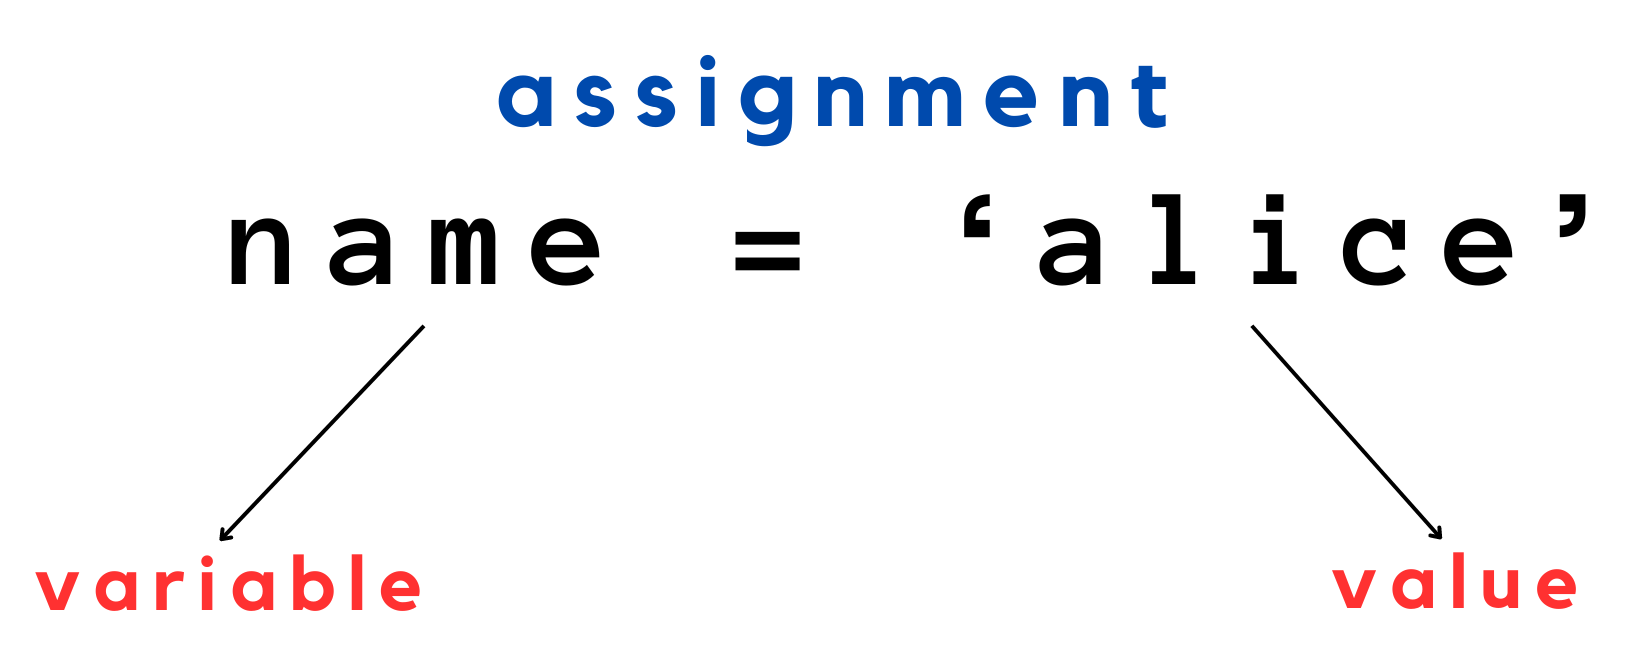
\includegraphics[width=0.7\textwidth]{../shared_assets/images/python_variable_structure.png}
	\caption{Struktur Variabel di Python}
	\label{fig:python-variable-structure}
\end{figure}

\noindent
Sumber gambar: \url{https://www.packetswitch.co.uk/python-variables-data-types/}

\subsection{Aturan Penamaan Variabel}

Pemberian nama variabel di Python harus mematuhi beberapa aturan penamaan yang disediakan oleh Python. Berikut adalah beberapa aturan penamaan variabel di Python:

\begin{itemize}
	\item Nama variabel harus dimulai dengan huruf atau underscore (\_).
	\item Nama variabel tidak boleh dimulai dengan angka.
	\item Nama variabel tidak boleh mengandung spasi.
	\item Nama variabel tidak boleh mengandung simbol.
	\item Nama variabel tidak boleh mengandung kata kunci (\textit{keyword}) yang sudah terdefinisi dalam Python, seperti \texttt{def}, \texttt{for}, \texttt{if}, \texttt{return}, dan sebagainya.
\end{itemize}

\subsection{Latihan Membuat Variabel}

Buat file baru dengan nama \textbf{variable.py} dan buat variabel dengan nama \textbf{nama}, \textbf{usia}, dan \textbf{berat_badan} dengan tipe data yang sesuai dan nilai-nilai yang sesuai. Kemudian cetak variabel tersebut.

\begin{lstlisting}[style=PythonStyle, caption={Kode Python: variable.py}]
nama = "Stefani Laurensia"
usia = 21
berat_badan = 50.2

print(nama)
print(usia)
print(berat_badan)
\end{lstlisting}

\subsection{Contoh Kesalahan Penamaan Variabel}

\begin{lstlisting}[style=PythonStyle, caption={Kode Python: variable.py}]
1angka = 200 # Nama variabel tidak boleh dimulai dengan angka
nama lengkap = "Budi" # Nama variabel tidak boleh mengandung spasi
gaji$ = 1000000 # Nama variabel tidak boleh mengandung simbol
class = "Informatika" # class merupakan kata kunci untuk membuat sebuah class di Python sehingga melanggar aturan di mana nama variabel tidak boleh mengandung kata kunci
\end{lstlisting}

\section{Konstanta}

Konstanta adalah variabel yang seharusnya nilainya tidak berubah selama program berjalan. Contohnya nilai \textbf{\textit{pi}} (3.14) atau gravitasi (9.81). Di Python, kita bisa menandai variabel sebagai Final dari modul \texttt{typing} untuk memberi tanda bahwa variabel tersebut dimaksudkan sebagai konstanta. Namun ada hal-hal yang perlu diperhatikan:
\begin{itemize}
	\item Python tidak memaksa variabel \texttt{Final} agar tidak bisa diubah.
	\item Penandaan \texttt{Final} hanya \textbf{memberi peringatan pada type checker}, bukan mencegah perubahan di runtime.
\end{itemize}

\subsection{Aturan Penamaan Konstanta}

Untuk menandakan bahwa sebuah variabel adalah konstanta, kita bisa menggunakan huruf besar untuk membedakan dengan variabel biasa. Hal ini mengikuti aturan penamaan variabel yang dibuat oleh Python (\href{https://peps.python.org/pep-0008/}{PEP 8 - Style Guide for Python Code}).

\subsection{Latihan Membuat Konstanta}

Buat file baru dengan nama \textbf{constant.py} dan buat konstanta dengan nama \textbf{PI} dan \textbf{GRAVITASI} dengan nilai yang sesuai. Kemudian cetak konstanta tersebut. Namun, berbeda dari bahasa pemrograman lain seperti C, C++, atau Java, di Python konstanta dapat diubah.
\begin{lstlisting}[style=PythonStyle, caption={Kode Python: constant.py}]
from typing import Final

PI: Final = 3.14
GRAVITASI: Final = 9.81

print(PI)
print(GRAVITASI)

GRAVITASI = 10 # Nilai masih tetap bisa berubah, tapi tidak disarankan
print(GRAVITASI)
\end{lstlisting}

\section{Tipe Data Dasar}

Tipe data merupakan jenis data yang bisa disimpan di program Python. Tipe data di Python memiliki banyak jenis, seperti \texttt{int}, \texttt{float}, \texttt{str}, \texttt{bool}, \texttt{list}, \texttt{tuple}, \texttt{dict}, dan \texttt{set}. Namun pada \textit{chapter} kali ini, kita akan fokus pada tipe data dasar, antara lain \texttt{int}, \texttt{float}, \texttt{str}, dan \texttt{bool}.
\newline \newline
Berdasarkan kelompoknya, tipe data dasar di Python dapat dibedakan menjadi 3 kelompok, antara lain:

\begin{enumerate}
\item \textbf{Numeric} (Angka)
\begin{enumerate}
\item \textbf{Integer} (bilangan bulat)
\begin{lstlisting}[style=PythonStyle]
usia = 18
jumlah_mahasiswa = 64
nomor_rumah = 88

suhu = -5
\end{lstlisting}

\item \textbf{Float} (bilangan desimal)
\begin{lstlisting}[style=PythonStyle]
koordinat_x = 5.5
koordinat_y = 7.8

saldo = 10.500.075
\end{lstlisting}
\end{enumerate}

\item \textbf{Teks} (Kata / Kalimat)
\begin{enumerate}
\item \textbf{String} (kumpulan karakter)
\begin{lstlisting}[style=PythonStyle]
nama = "John"
quote = 'Programmer: A machine that turns coffee into code'
pesan_email = """
Kepada Yth. John Doe,

Terima kasih atas pesanan anda.
"""
\end{lstlisting}
\end{enumerate}

\item \textbf{Boolean} (Benar atau Salah)
\begin{lstlisting}[style=PythonStyle]
is_married = False
is_single = True
\end{lstlisting}
\end{enumerate}

\section{Konversi Tipe Data (\textit{Type Casting})}

Kadang kita perlu mengubah tipe data dari satu jenis ke jenis lain agar Python bisa memprosesnya dengan benar.
Misal, input dari pengguna melalui fungsi \texttt{input()} selalu mengembalikan tipe data string (str), tapi kita ingin melakukan perhitungan angka, maka kita harus mengubahnya menjadi int atau float.

\begin{table}[h!]
\centering
\begin{tabular}{|c|c|c|}
\hline
\textbf{Fungsi} & \textbf{Keterangan} & \textbf{Contoh} \\
\hline
int() & Ubah menjadi bilangan bulat & int("10") → 10 \\
\hline
float() & Ubah menjadi bilangan desimal & float("3.14") → 3.14 \\
\hline
str() & Ubah menjadi teks & str(10) → "10" \\
\hline
bool() & Ubah menjadi True/False & bool(0) → False, bool(5) → True \\
\hline
\end{tabular}
\caption{Fungsi Untuk Konversi Tipe Data di Python}
\end{table}

\subsection{Latihan Konversi Tipe Data}

\begin{lstlisting}[style=PythonStyle, caption={Kode Python: string_to_int.py}]
usia = input("Masukkan usia Anda: ")
print("Tipe data sebelum konversi:", type(usia)) # Menampilkan tipe data sebelum konversi

usia = int(usia) # Konversi tipe data string menjadi integer
print("Tipe data setelah konversi:", type(usia)) # Menampilkan tipe data setelah konversi

usia_lima_tahun_kemudian = usia + 5 # Perhitungan usia 5 tahun kemudian
print("Usia 5 tahun kemudian:", usia_lima_tahun_kemudian)
\end{lstlisting}

\begin{lstlisting}[style=PythonStyle, caption={Kode Python: string_to_float.py}]
angka_str = "45.67"
print("Sebelum konversi:", angka_str, type(angka_str))

angka_float = float(angka_str)
print("Setelah konversi ke float:", angka_float, type(angka_float))
\end{lstlisting}

\begin{lstlisting}[style=PythonStyle, caption={Kode Python: int_to_float.py}]
angka_int = 10
print("Sebelum konversi:", angka_int, type(angka_int))

angka_float = float(angka_int)
print("Setelah konversi ke float:", angka_float, type(angka_float))
\end{lstlisting}

\begin{lstlisting}[style=PythonStyle, caption={Kode Python: float_to_int.py}]
angka_float = 3.99
print("Sebelum konversi:", angka_float, type(angka_float))

angka_int = int(angka_float)
print("Setelah konversi ke integer:", angka_int, type(angka_int))
\end{lstlisting}

\subsection{Kesalahan dalam Konversi Tipe Data}
Meskipun Python menyediakan fungsi bawaan untuk mengubah tipe data (\texttt{int()}, \texttt{float()}, \texttt{str()}, \texttt{bool()}), \textbf{tidak semua konversi bisa dilakukan dengan sukses}. Jika nilai yang dikonversi tidak sesuai dengan tipe data tujuan, maka program akan menghasilkan \textbf{error}. Berikut adalah contoh kesalahan dalam konversi tipe data:

\begin{lstlisting}[style=PythonStyle]
# String huruf → Integer
huruf = "abc"
huruf_integer = int(huruf) 
# Output: ValueError: invalid literal for int() with base 10: 'abc'

# String bilangan desimal → Integer
angka_str = "12.34"
angka_int = int(angka_str)  
# Output: ValueError: invalid literal for int() with base 10: '12.34'
\end{lstlisting}

Perhatikan pada contoh di atas bahwa program akan menghasilkan \textbf{error} ketika nilai yang dikonversi tidak sesuai dengan tipe data tujuan. Hal ini diakibatkan karena fungsi \texttt{int()} hanya dapat mengubah \textbf{string yang berisi bilangan bulat} menjadi tipe data \texttt{integer}.
\par
Apabila string berisi karakter non-angka (misalnya \texttt{"abc"}) atau bilangan desimal (misalnya \texttt{"12.34"}), maka Python tidak dapat memprosesnya langsung sebagai \texttt{integer} dan akan menampilkan pesan \texttt{ValueError}. Untuk kasus bilangan desimal dalam bentuk string, diperlukan dua tahap konversi, yaitu:
\begin{enumerate}
	\item Konversi string ke tipe data \texttt{float}.
	\item Konversi tipe data \texttt{float} ke tipe data \texttt{integer}.
\end{enumerate}

\section{Soal Latihan}

Berikut adalah beberapa soal latihan tambahan untuk menguji pemahaman Anda mengenai konsep variabel, konstanta tipe data, dan konversi tipe data yang telah dipelajari:
\begin{enumerate}
\item \textbf{Soal 1:} Buat program bernama \texttt{luas_persegi_panjang.py} yang meminta pengguna memasukan nilai panjang dan lebar persegi panjang, kemudian program harus bisa menghitung dan mencetak luas persegi panjang tersebut.
\newline \newline
\textbf{Hint:} Gunakan operator perkalian \texttt{*} untuk menghitung luas.

\item \textbf{Soal 2:} Buat program bernama \texttt{luas_lingkaran.py} yang meminta pengguna memasukan nilai jari-jari lingkaran. Program harus menampung nilai konstanta \textbf{\textit{pi}} mengikuti standar \textit{best practice} dari Python dan bisa menghitung sekaligus mencetak luas lingkaran tersebut.

\item \textbf{Soal 3:} Buat program bernama \texttt{tebak_usia.py} yang meminta pengguna memasukkan tahun lahirnya. Program harus:
\begin{enumerate}
    \item Menyimpan tahun lahir di variabel.
    \item Mengubah input dari string menjadi integer.
    \item Menghitung umur dengan mengurangi tahun saat ini dengan tahun lahir yang dimasukan oleh pengguna.
    \item Menampilkan pesan seperti: "Kamu berusia [umur] tahun."
\end{enumerate}

\textbf{Hint:} Gunakan operator pengurangan \texttt{-} untuk menghitung usia saat ini.

\end{enumerate}
	\chapter{Operator dan Pengkondisian}

\section{Operator}
Operator adalah karakter khusus yang digunakan untuk melakukan operasi terhadap variabel dan nilai. Di Python terdapat berbagai jenis operator, namun pada chapter ini kita hanya akan membahas beberapa operator yang paling umum digunakan, yaitu:

\begin{enumerate}
    \item Operator Aritmatika
    \item Operator \textit{Assignment}
    \item Operator Perbandingan
    \item Operator Logika
    \item Operator \textit{Membership}
\end{enumerate}

\subsection{Operator Aritmatika}
\begin{frame}[fragile]{Operator Aritmatika di Python}
Operator ini dipakai untuk melakukan operasi dasar dalam matematika, seperti penjumlahan, pengurangan, perkalian, pembagian, dan sebagainya.

\end{frame}

\begin{table}[H]
\centering
\begin{tabular}{|c|c|c|}
\hline
\textbf{Operator} & \textbf{Keterangan} \\
\hline
\texttt{+} & Operator penjumlahan \\
\hline
\texttt{-} & Operator pengurangan \\
\hline
\texttt{*} & Operator perkalian \\
\hline
\texttt{/} & Operator pembagian \\
\hline
\texttt{//} & Operator pembagian bulat (\textit{floor division}) \\
\hline
\texttt{\%} & Operator modulus (sisa hasil bagi) \\
\hline
\texttt{**} & Operator perpangkatan \\
\hline
\end{tabular}
\caption{Daftar Operator Aritmatika di Python}
\end{table}

Berikut adalah contoh penggunaan operator aritmatika dalam Python:
\begin{lstlisting}[style=PythonStyle, caption={Kode Python: arithmetic_operator.py}]
a = 5
b = 2

print("a + b =", a + b)
print("a - b =", a - b)
print("a * b =", a * b)
print("a / b =", a / b)
print("a // b =", a // b)
print("a % b =", a % b)
print("a ** b =", a ** b)
\end{lstlisting}

Kode di atas mendemonstrasikan berbagai operasi aritmatika yang dapat dilakukan di Python menggunakan operator bawaan. Berikut adalah penjelasan dari setiap operasi:
\begin{itemize}
    \item Penjumlahan (+)
    \begin{itemize}
        \item \texttt{print("a + b =", a + b)} menghasilkan penjumlahan dari \texttt{a} dan \texttt{b}, yaitu $5 + 2 = 7$.
    \end{itemize}

    \item Pengurangan (-)
    \begin{itemize}
        \item \texttt{print("a - b =", a - b)} menghasilkan pengurangan dari \texttt{a} dan \texttt{b}, yaitu $5 - 2 = 3$.
    \end{itemize}

    \item Perkalian (*)
    \begin{itemize}
        \item \texttt{print("a * b =", a * b)} menghasilkan perkalian dari \texttt{a} dan \texttt{b}, yaitu $5 \times 2 = 10$.
    \end{itemize}

    \item Pembagian (/)
    \begin{itemize}
        \item \texttt{print("a / b =", a / b)} menghasilkan pembagian dari \texttt{a} dan \texttt{b}, yaitu $5 / 2 = 2.5$.
    \end{itemize}

    \item \textit{Floor Division} (//)
    \begin{itemize}
        \item \texttt{print("a // b =", a // b)} menghasilkan pembagian bulat dari \texttt{a} dan \texttt{b} dengan pembulatan ke bawah, yaitu $5 // 2 = 2$.
    \end{itemize}

    \item Modulo (\%)
    \begin{itemize}
        \item \texttt{print("a \% b =", a \% b)} menghasilkan sisa hasil bagi dari \texttt{a} dibagi \texttt{b}, yaitu $5 \% 2 = 1$.
    \end{itemize}

    \item Perpangkatan (**)
    \begin{itemize}
        \item \texttt{print("a ** b =", a ** b)} menghasilkan \texttt{a} dipangkatkan dengan \texttt{b}, yaitu $5^2 = 25$.
    \end{itemize}
\end{itemize}

\subsection{Operator \textit{Assignment}}
Operator \textit{assignment} adalah operator yang digunakan untuk memberikan nilai pada variabel. 
Selain \textit{assignment} dasar dengan tanda sama dengan (\texttt{=}), Python juga menyediakan operator 
\textit{assignment} gabungan (\textit{augmented assignment}) yang mengombinasikan operasi aritmatika dengan assignment.

\begin{table}[H]
\centering
\begin{tabular}{|c|c|}
\hline
\textbf{Operator} & \textbf{Keterangan} \\
\hline
\texttt{=} & Assignment, memberikan nilai ke variabel \\
\hline
\texttt{+=} & Penjumlahan sekaligus assignment (\texttt{x += y} $\Rightarrow$ \texttt{x = x + y}) \\
\hline
\texttt{-=} & Pengurangan sekaligus assignment (\texttt{x -= y} $\Rightarrow$ \texttt{x = x - y}) \\
\hline
\texttt{*=} & Perkalian sekaligus assignment (\texttt{x *= y} $\Rightarrow$ \texttt{x = x * y}) \\
\hline
\texttt{/=} & Pembagian sekaligus assignment (\texttt{x /= y} $\Rightarrow$ \texttt{x = x / y}) \\
\hline
\texttt{//=} & Floor division sekaligus assignment (\texttt{x //= y} $\Rightarrow$ \texttt{x = x // y}) \\
\hline
\texttt{\%=} & Modulo sekaligus assignment (\texttt{x \%= y} $\Rightarrow$ \texttt{x = x \% y}) \\
\hline
\texttt{**=} & Perpangkatan sekaligus assignment (\texttt{x **= y} $\Rightarrow$ \texttt{x = x ** y}) \\
\hline
\end{tabular}
\caption{Daftar Operator Assignment di Python}
\end{table}

Berikut adalah contoh penggunaan operator assignment dalam Python:
\begin{lstlisting}[style=PythonStyle, caption={Kode Python: assignment_operator.py}]
x = 10
print("x =", x)

x += 5
print("x += 5 ->", x)

x -= 3
print("x -= 3 ->", x)

x *= 2
print("x *= 2 ->", x)

x /= 4
print("x /= 4 ->", x)

x //= 2
print("x //= 2 ->", x)

x %= 3
print("x %= 3 ->", x)

x **= 2
print("x **= 2 ->", x)
\end{lstlisting}

Kode di atas mendemonstrasikan berbagai operator assignment yang dapat digunakan di Python. 
Berikut adalah penjelasan dari setiap operator:
\begin{itemize}
    \item Assignment (=)
    \begin{itemize}
        \item \texttt{x = 10} memberikan nilai $10$ ke variabel \texttt{x}.
    \end{itemize}

    \item Penjumlahan Assignment (+=)
    \begin{itemize}
        \item \texttt{x += 5} sama dengan \texttt{x = x + 5}. Jika sebelumnya $x = 10$, maka setelah operasi ini $x = 15$.
    \end{itemize}

    \item Pengurangan Assignment (-=)
    \begin{itemize}
        \item \texttt{x -= 3} sama dengan \texttt{x = x - 3}. Jika $x = 15$, maka hasilnya $x = 12$.
    \end{itemize}

    \item Perkalian Assignment (*=)
    \begin{itemize}
        \item \texttt{x *= 2} sama dengan \texttt{x = x * 2}. Jika $x = 12$, maka hasilnya $x = 24$.
    \end{itemize}

    \item Pembagian Assignment (/=)
    \begin{itemize}
        \item \texttt{x /= 4} sama dengan \texttt{x = x / 4}. Jika $x = 24$, maka hasilnya $x = 6.0$.
    \end{itemize}

    \item Floor Division Assignment (//=)
    \begin{itemize}
        \item \texttt{x //= 2} sama dengan \texttt{x = x // 2}. Jika $x = 6.0$, maka hasilnya $x = 3.0$.
    \end{itemize}

    \item Modulo Assignment (\%=)
    \begin{itemize}
        \item \texttt{x \%= 3} sama dengan \texttt{x = x \% 3}. Jika $x = 3.0$, maka hasilnya $x = 0.0$.
    \end{itemize}

    \item Perpangkatan Assignment (**=)
    \begin{itemize}
        \item \texttt{x **= 2} sama dengan \texttt{x = x ** 2}. Jika $x = 0.0$, maka hasilnya tetap $0.0$.
    \end{itemize}
\end{itemize}

\subsection{Operator Perbandingan}
Operator perbandingan digunakan untuk membandingkan dua nilai. 
Hasil dari operator ini selalu berupa nilai boolean (\texttt{True} atau \texttt{False}).

\begin{table}[H]
\centering
\begin{tabular}{|c|c|}
\hline
\textbf{Operator} & \textbf{Keterangan} \\
\hline
\texttt{==} & Sama dengan \\
\hline
\texttt{!=} & Tidak sama dengan \\
\hline
\texttt{>} & Lebih besar dari \\
\hline
\texttt{<} & Lebih kecil dari \\
\hline
\texttt{>=} & Lebih besar atau sama dengan \\
\hline
\texttt{<=} & Lebih kecil atau sama dengan \\
\hline
\end{tabular}
\caption{Daftar Operator Perbandingan di Python}
\end{table}

\begin{lstlisting}[style=PythonStyle, caption={Kode Python: comparison_operator.py}]
a = 5
b = 2

print("a == b:", a == b)
print("a != b:", a != b)
print("a > b:", a > b)
print("a < b:", a < b)
print("a >= b:", a >= b)
print("a <= b:", a <= b)
\end{lstlisting}

\subsection{Operator Logika}
Operator logika digunakan untuk menggabungkan ekspresi boolean.

\begin{table}[H]
\centering
\begin{tabular}{|c|c|}
\hline
\textbf{Operator} & \textbf{Keterangan} \\
\hline
\texttt{and} & Bernilai \texttt{True} jika kedua kondisi bernilai benar \\
\hline
\texttt{or} & Bernilai \texttt{True} jika salah satu kondisi bernilai benar \\
\hline
\texttt{not} & Membalikkan nilai boolean (True menjadi False, sebaliknya) \\
\hline
\end{tabular}
\caption{Daftar Operator Logika di Python}
\end{table}

\begin{lstlisting}[style=PythonStyle, caption={Kode Python: logical_operator.py}]
x = True
y = False

print("x and y:", x and y)
print("x or y:", x or y)
print("not x:", not x)
\end{lstlisting}

\subsection{Operator \textit{Membership}}
Operator \textit{membership} digunakan untuk memeriksa apakah suatu nilai (biasanya berupa karakter atau substring) 
terdapat di dalam sebuah string. Hasil dari operasi ini berupa nilai boolean (\texttt{True} atau \texttt{False}).

\begin{table}[H]
\centering
\begin{tabular}{|c|c|}
\hline
\textbf{Operator} & \textbf{Keterangan} \\
\hline
\texttt{in} & Bernilai \texttt{True} jika nilai ada di dalam string \\
\hline
\texttt{not in} & Bernilai \texttt{True} jika nilai tidak ada di dalam string \\
\hline
\end{tabular}
\caption{Daftar Operator \textit{Membership} di Python}
\end{table}

\begin{lstlisting}[style=PythonStyle, caption={Kode Python: membership_operator.py}]
text = "Python Programming"

print("'Py' in text:", "Py" in text)         # True
print("'Java' in text:", "Java" in text)     # False
print("'Java' not in text:", "Java" not in text) # True
print("'P' in text:", "P" in text)           # True
\end{lstlisting}

\section{Pengkondisian}
Pengkondisian adalah konsep penting dalam pemrograman yang memungkinkan pengambilan keputusan berdasarkan kondisi tertentu. Di Python, pengkondisian bisa diimplementasikan menggunakan beberapa struktur dasar seperti if, elif, else, match, dan operator ternary.

\subsection{If}
If digunakan untuk mengeksekusi blok kode tertentu hanya jika kondisi yang diberikan bernilai true. Bentuk dasarnya adalah:

\begin{lstlisting}[style=PythonStyle, caption={Bentuk dasar if}]
if kondisi:
    # Blok kode yang akan dieksekusi jika kondisi bernilai true
\end{lstlisting}

Contoh Penggunaan:

\begin{lstlisting}[style=PythonStyle, caption={Kode Python: if_statement.py}]
nilai = 75
if nilai >= 70:
    print("Lulus")
\end{lstlisting}

\subsection{If-Else}
If-else memungkinkan kita untuk menentukan blok kode alternatif yang akan dijalankan jika kondisi tidak terpenuhi. Bentuk dasarnya adalah:

\begin{lstlisting}[style=PythonStyle, caption={Bentuk dasar if-else}]
if kondisi:
    # Blok kode yang akan dieksekusi jika kondisi bernilai true
else:
    # Blok kode yang akan dieksekusi jika kondisi bernilai false
\end{lstlisting}

Contoh Penggunaan:

\begin{lstlisting}[style=PythonStyle, caption={Kode Python: if_else_statement.py}]
nilai = 65
if nilai >= 70:
    print("Lulus")
else:
    print("Tidak Lulus")
\end{lstlisting}

\subsection{If-Elif-Else (Percabangan Multi Kondisi)}
If-elif-else memungkinkan kita untuk menentukan beberapa kondisi dan blok kode yang akan dijalankan jika kondisi tersebut bernilai true. Bentuk dasarnya adalah:

\begin{lstlisting}[style=PythonStyle, caption={Bentuk dasar if-elif-else}]
if kondisi1:
    # Blok kode yang akan dieksekusi jika kondisi1 bernilai true
elif kondisi2:
    # Blok kode yang akan dieksekusi jika kondisi2 bernilai true
else:
    # Blok kode yang akan dieksekusi jika kondisi1 dan kondisi2 bernilai false
\end{lstlisting}

Contoh Penggunaan:

\begin{lstlisting}[style=PythonStyle, caption={Kode Python: if_elif_else_statement.py}]
nilai = 65
if nilai >= 90:
    print("A")
elif nilai >= 80:
    print("B")
elif nilai >= 70:
    print("C")
else:
    print("D")
\end{lstlisting}

\subsection{\textit{Nested-If}}
\textit{Nested-if} adalah struktur if yang digunakan untuk membuat blok kode yang bersarang. Bentuk dasarnya adalah:

\begin{lstlisting}[style=PythonStyle, caption={Bentuk dasar nested-if}]
if kondisi1:
    # Blok kode yang akan dieksekusi jika kondisi1 bernilai true
    if kondisi2:
        # Blok kode yang akan dieksekusi jika kondisi2 bernilai true
    else:
        # Blok kode yang akan dieksekusi jika kondisi2 bernilai false
else:
    # Blok kode yang akan dieksekusi jika kondisi1 bernilai false
\end{lstlisting}

Contoh Penggunaan:

\begin{lstlisting}[style=PythonStyle, caption={Kode Python: nested_if_statement.py}]
usia = 25
punya_surat_izin_mengemudi = True

if usia >= 18:  # Kondisi luar: cek apakah usia sudah 18 tahun ke atas
    print("Kamu sudah dewasa.")
    if punya_surat_izin_mengemudi:  # Kondisi dalam: cek apakah sudah punya SIM
        print("Kamu boleh mengemudi.")
    else:
        print("Kamu sudah dewasa, tapi belum punya SIM.")
else:
    print("Kamu belum dewasa.")
\end{lstlisting}

\subsection{\textit{Match}}
Sejak Python 3.10, tersedia struktur kontrol baru bernama \texttt{match} yang mirip dengan \texttt{switch-case} di bahasa pemrograman lain. Dengan \texttt{match}, kita dapat mencocokkan sebuah nilai terhadap beberapa pola sekaligus. Bentuk dasarnya adalah:

\begin{lstlisting}[style=PythonStyle, caption={Bentuk dasar match}]
match variabel / value:
    case pola1:
        # blok kode jika sesuai pola1
    case pola2:
        # blok kode jika sesuai pola2
    case _:
        # blok kode default jika tidak ada yang cocok
\end{lstlisting}

Berikut contoh penggunaannya:

\begin{lstlisting}[style=PythonStyle, caption={Kode Python: match.py}]
hari = "Senin"

match hari:
    case "Senin":
        print("Awal minggu, semangat kerja!")
    case "Jumat":
        print("Akhir minggu, hampir libur!")
    case _:
        print("Hari biasa.")
\end{lstlisting}

\subsection{Operator Ternary (\textit{Conditional Expression})}

Python mendukung bentuk singkat dari struktur \texttt{if-else} yang disebut dengan
\textit{conditional expression} atau sering dikenal sebagai \textit{ternary operator}.
Sintaksnya adalah:

\begin{lstlisting}[style=PythonStyle, caption={Bentuk dasar ternary operator di Python}]
nilai_jika_true if kondisi else nilai_jika_false
\end{lstlisting}

Contoh penggunaannya:

\begin{lstlisting}[style=PythonStyle, caption={Kode Python: ternary_operator.py}]
usia = 20

status = "Dewasa" if usia >= 18 else "Anak-anak"

print("Status:", status)
\end{lstlisting}

Kode di atas setara dengan:

\begin{lstlisting}[style=PythonStyle]
if usia >= 18:
    status = "Dewasa"
else:
    status = "Anak-anak"
\end{lstlisting}

\section{Latihan}
Berikut adalah beberapa latihan yang dapat Anda coba untuk memperdalam pemahaman tentang program Python yang telah dibahas:

\begin{enumerate}
\item \textbf{Latihan 1:} Buatlah program yang menerima input 5 nilai asesmen mahasiswa yang kemudian dihitung rata-ratanya. Berdasarkan rata-rata tersebut buatlah pengkondisian menggunakan \textit{if-elif-else statement} untuk menentukan grade yang sesuai dengan ketentuan:
\begin{itemize}
    \item Grade A jika rata-rata berada di \textit{range} 90,00 - 100
    \item Grade A- jika rata-rata berada di \textit{range} 85,00 - 89,99
    \item Grade B+ jika rata-rata berada di \textit{range} 80,00 - 84,99
    \item Grade B jika rata-rata berada di \textit{range} 75,00 - 79,99
    \item Grade B- jika rata-rata berada di \textit{range} 70,00 - 74,99
    \item Grade C+ jika rata-rata berada di \textit{range} 65,00 - 69,99
    \item Grade C jika rata-rata berada di \textit{range} 60,00 - 64,99
    \item Grade D jika rata-rata berada di \textit{range} 55,00 - 59,99
    \item Grade E jika rata-rata kurang dari 49,99
\end{itemize}

\item \textbf{Latihan 2:} Buatlah program untuk menghitung \textit{Body Mass Index} (BMI) seseorang dengan rumus:

\[
BMI = \frac{berat \ (kg)}{(tinggi \ (m))^2}
\]

\begin{itemize}
    \item Program meminta input berat badan (kg) dan tinggi badan (cm).
    \item Konversikan tinggi badan dari cm menjadi meter.
    \item Hitung nilai BMI menggunakan rumus di atas.
    \item Kategorikan hasilnya dengan \texttt{if-elif-else}:
    \begin{itemize}
        \item $<$ 18.5 : \texttt{Kurus}
        \item 18.5 -- 24.9 : \texttt{Normal}
        \item 25 -- 29.9 : \texttt{Overweight}
        \item $\geq$ 30 : \texttt{Obesitas}
    \end{itemize}
\end{itemize}

\item \textbf{Latihan 3:} Modifikasi program BMI pada Latihan 2 dengan ketentuan berikut:
\begin{itemize}
    \item Program tetap meminta input berat badan (kg) dan tinggi badan (cm).
    \item Konversikan tinggi badan dari cm ke meter, lalu hitung nilai BMI.
    \item Gunakan struktur \texttt{if-elif-else} untuk menentukan kategori BMI:
    \begin{itemize}
        \item $<$ 18.5 : \texttt{"kurus"}
        \item 18.5 -- 24.9 : \texttt{"normal"}
        \item 25 -- 29.9 : \texttt{"overweight"}
        \item $\geq$ 30 : \texttt{"obesitas"}
    \end{itemize}
    \item Setelah kategori ditentukan, gunakan \texttt{match-case} untuk menampilkan pesan sesuai kategori:
    \begin{itemize}
        \item \texttt{"kurus"} : tampilkan pesan untuk memperhatikan asupan gizi
        \item \texttt{"normal"} : tampilkan pesan untuk mempertahankan pola hidup sehat
        \item \texttt{"overweight"} : tampilkan pesan untuk mulai menjaga pola makan
        \item \texttt{"obesitas"} : tampilkan pesan untuk konsultasi ke dokter
    \end{itemize}
\end{itemize}


\item \textbf{Latihan 4:} Buatlah program autentikasi sederhana yang meminta pengguna untuk memasukkan email dan password. Program harus memenuhi kriteria sebagai berikut:
\begin{itemize}
    \item Email harus berupa alamat email dengan domain \texttt{pradita.ac.id}
    \item Password harus memiliki panjang minimal 8 karakter
    \item Gunakan \textit{data dummy} (statis), misalnya email \texttt{mahasiswa@pradita.ac.id} dan password \texttt{password123}, untuk proses pencocokan
\end{itemize}

\item \textbf{Latihan 5:} Buatlah program kalkulator sederhana yang:
\begin{itemize}
    \item Meminta pengguna memilih operasi aritmatika yang ingin dilakukan (\texttt{+}, \texttt{-}, \texttt{*}, \texttt{/})
    \item Meminta pengguna memasukkan dua buah angka
    \item Menampilkan hasil perhitungan sesuai operasi yang dipilih
    \item Jika pengguna memasukkan operasi yang tidak valid, tampilkan pesan error
\end{itemize}

\end{enumerate}
	\chapter{Fungsi and Modul}

\section{Fungsi}
Fungsi adalah blok kode terorganisir yang memiliki nama tertentu dan dapat dipanggil berulang kali untuk melakukan tugas spesifik, mengurangi redundansi kode, dan mempermudah pengelolaan program. Fungsi membantu kita menulis kode yang lebih rapi, modular, dan mudah dipelihara.

\subsection{Fungsi Dasar Tanpa Parameter}

Fungsi sederhana yang tidak menerima parameter dan tidak mengembalikan nilai. Fungsi ini hanya menjalankan perintah tertentu.

\begin{lstlisting}[style=PythonStyle, caption={Kode Python: basic_function.py}]
def greet():
    print("Halo, selamat datang!")

# Memanggil fungsi
greet()
\end{lstlisting}

\subsection{Fungsi dengan Parameter}

Fungsi bisa memiliki parameter. Dengan adanya parameter, suatu nilai bisa di-sisipkan ke dalam fungsi secara dinamis saat pemanggilannya.

Parameter sendiri merupakan istilah untuk variabel yang menempel pada fungsi, yang mengharuskan kita untuk menyisipkan nilai pada parameter tersebut saat pemanggilan fungsi.

\begin{lstlisting}[style=PythonStyle, caption={Kode Python: parameter_function.py}]
def greet_with_name(nama):
    print(f"Halo, {nama}!")

# Memanggil fungsi dengan argumen
greet_with_name("Jessie")
\end{lstlisting}

\subsection{Fungsi dengan Nilai Kembalian (Return Value)}

Fungsi dapat mengembalikan hasil yang dapat disimpan atau digunakan dalam perhitungan lain.

\subsubsection{Return Nilai Tunggal}
\begin{lstlisting}[style=PythonStyle, caption={Kode Python: function_with_single_return.py}]
def add(a, b):
    return a + b

summation_result = add(5, 3)
print(summation_result)  # Output: 8
\end{lstlisting}

\subsubsection{Return Lebih dari Satu Nilai}
\begin{lstlisting}[style=PythonStyle, caption={Kode Python: function_with_multiple_return.py}]
def operate(a, b):
    return a + b, a * b

sum_result, product_result = operate(4, 5)
print(sum_result)     # 9
print(product_result) # 20
\end{lstlisting}

\subsection{Fungsi dengan Parameter Default}

Fungsi dapat memiliki nilai default untuk parameter jika argumen tidak diberikan saat pemanggilan.

\begin{lstlisting}[style=PythonStyle, caption={Kode Python: function_with_default_parameter.py}]
def greet_you(name="Friend"):
    print(f"Hello, {name}!")

greet_you()        # Output: Hello, Friend!
greet_you("Andrew")  # Output: Hello, Andrew!
\end{lstlisting}

\subsection{Fungsi dengan Argumen Keyword dan Positional}
Fungsi di Python bisa dipanggil menggunakan positional arguments atau keyword arguments. Positional argument adalah istilah untuk urutan parameter/argument fungsi. Pengisian argument saat pemanggilan fungsi harus urut sesuai dengan deklarasi parameternya. Keyword argument atau named argument adalah metode pengisian argument pemanggilan fungsi disertai nama parameter yang ditulis secara jelas (eksplisit).

\begin{lstlisting}[style=PythonStyle, caption={Kode Python: function_with_keyword_and_positional.py}]
def student_info(name, age, major):
    print(f"{name}, {age} years old, majoring in {major}")

# Positional arguments
student_info("Delta", 20, "Computer Science")

# Keyword arguments
student_info(major="Information Systems", name="Echo", age=21)
\end{lstlisting}

\subsection{Fungsi dengan Jumlah Argumen Variabel}

Jika jumlah argumen tidak pasti, kita bisa menggunakan \texttt{*args}.

\begin{lstlisting}[style=PythonStyle, caption={Kode Python: function_with_variable_arguments.py}]
def sum_numbers(*numbers):
    total = sum(numbers)
    print(f"Total: {total}")

sum_numbers(1, 2, 3, 4)  # Output: Total: 10
sum_numbers(5, 6, 7)     # Output: Total: 18
\end{lstlisting}

\subsection{Fungsi Rekursif}

Fungsi yang memanggil dirinya sendiri. Biasanya digunakan untuk masalah yang dapat dipecah menjadi sub-masalah.

\begin{lstlisting}[style=PythonStyle, caption={Kode Python: recursive_function.py}]
def factorial(n):
    if n == 0 or n == 1:
        return 1
    else:
        return n * factorial(n-1)

print(factorial(5))  # Output: 120
\end{lstlisting}

\section{Modul}

Modul adalah file Python (\texttt{.py}) yang berisi kode seperti fungsi, variabel, atau kelas, yang bisa digunakan kembali di program lain. Modul membantu memecah program menjadi bagian-bagian yang lebih kecil dan terstruktur.

\subsection{Membuat Modul}

Modul sendiri dibuat dengan membuat file Python baru. Misalnya kita buat file \texttt{math_operations.py}:

\begin{lstlisting}[style=PythonStyle, caption={Kode Python: math_operations.py}]
def add(a, b):
    """Mengembalikan hasil penjumlahan a + b"""
    return a + b

def subtract(a, b):
    """Mengembalikan hasil pengurangan a - b"""
    return a - b

def multiply(a, b):
    """Mengembalikan hasil perkalian a * b"""
    return a * b

def divide(a, b):
    """Mengembalikan hasil pembagian a / b"""
    if b == 0:
        return "Error: Division by zero!"
    return a / b

def power(a, b):
    """Mengembalikan hasil a pangkat b"""
    return a ** b
\end{lstlisting}

Lalu kita bisa menggunakan modul ini di file program lain:

\begin{lstlisting}[style=PythonStyle, caption={Kode Python: calculator.py}]
import math_operations

print(math_operations.add(5, 3))        # Output: 8
print(math_operations.subtract(10, 4))  # Output: 6
print(math_operations.multiply(2, 7))   # Output: 14
print(math_operations.divide(10, 2))    # Output: 5.0
print(math_operations.power(3, 4))      # Output: 81
\end{lstlisting}

\subsection{Mengimpor Modul dengan Alias}

Kita bisa memberi nama alias saat mengimpor modul agar lebih ringkas:

\begin{lstlisting}[style=PythonStyle, caption={Kode Python: calculator.py}]
import math_operations as mo

print(mo.add(5, 3))        # Output: 8
print(mo.subtract(10, 4))  # Output: 6
print(mo.multiply(2, 7))   # Output: 14
print(mo.divide(10, 2))    # Output: 5.0
print(mo.power(3, 4))      # Output: 81
\end{lstlisting}

\subsection{Menaruh Modul dalam Folder}

Selain membuat modul di satu file, kita juga bisa menaruh modul di dalam folder supaya lebih rapi. Misalnya:

\begin{verbatim}
project/
│
├── main.py
└── utils/
└── string_utils.py
\end{verbatim}

Isi \texttt{string_utils.py} misalnya:

\begin{lstlisting}[style=PythonStyle, caption={Kode Python: utils/string_utils.py}]
def to_upper(text):
return text.upper()

def to_lower(text):
return text.lower()
\end{lstlisting}

Di \texttt{main.py}, kita bisa mengimpor modul ini dari folder \texttt{utils}:

\begin{lstlisting}[style=PythonStyle, caption={Kode Python: main.py}]
from utils import string_utils

print(string_utils.to_upper("Python")) # Output: PYTHON
print(string_utils.to_lower("Python")) # Output: python
\end{lstlisting}

\subsection{Best Practice: Paket dengan __init__.py}

Untuk project yang lebih besar atau modul yang akan digunakan di banyak file, sebaiknya folder modul dijadikan \textbf{package} dengan menambahkan file __init__.py:

\begin{verbatim}
project/
│
├── main.py
└── utils/
├── __init__.py
└── string_utils.py
\end{verbatim}

Dengan __init__.py, Python mengenali folder sebagai package.

Cara import tetap sama:

\begin{lstlisting}[style=PythonStyle]
from utils import string_utils
\end{lstlisting}

\subsubsection{Modul Bawaan Python}

Python memiliki banyak modul bawaan yang bisa langsung digunakan tanpa instalasi. Beberapa modul bawaan yang sering dipakai antara lain:

\texttt{math} — untuk operasi matematika, seperti akar, pangkat, atau konstanta \(\pi\).

\texttt{random} — untuk menghasilkan angka acak.

\texttt{datetime} — untuk mengelola tanggal dan waktu.

\texttt{os} — untuk berinteraksi dengan sistem operasi, misal folder, file, path.

Contoh penggunaan modul bawaan:

\begin{lstlisting}[style=PythonStyle, caption={Kode Python: math_module.py}]
import math

print(math.sqrt(16)) # Output: 4.0
print(math.pi) # Output: 3.141592653589793
\end{lstlisting}

\begin{lstlisting}[style=PythonStyle, caption={Kode Python: random_module.py}]
import random

print(random.randint(1, 10)) # Output: angka acak antara 1 sampai 10
\end{lstlisting}

\begin{lstlisting}[style=PythonStyle, caption={Kode Python: datetime_module.py}]
from datetime import date

today = date.today()
print(today) # Output: tanggal hari ini, misal 2025-09-20
\end{lstlisting}

\subsubsection{Mengimpor Fungsi atau Variabel Tertentu}

Jika hanya membutuhkan beberapa fungsi/variabel dari modul, bisa langsung diimpor:

\begin{lstlisting}[style=PythonStyle]
from math import sqrt, pi

print(sqrt(36)) # Output: 6.0
print(pi) # Output: 3.141592653589793
\end{lstlisting}

\section{Latihan}

\begin{enumerate}
    \item \textbf{Soal 1:} Buatlah program yang meminta pengguna memasukan nilai (minimal 5 input), kemudian klasifikasikan nilai tersebut sesuai dengan ketentuan berikut:
    \begin{enumerate}
        \item Jika nilai lebih besar atau sama dengan 80, maka klasifikasi \texttt{A}
        \item Jika nilai lebih besar atau sama dengan 70, maka klasifikasi \texttt{B}
        \item Jika nilai lebih besar atau sama dengan 60, maka klasifikasi \texttt{C}
        \item Jika nilai lebih besar atau sama dengan 50, maka klasifikasi \texttt{D}
        \item Jika nilai lebih kecil dari 50, maka klasifikasi \texttt{E}
    \end{enumerate}
    Buatkan program dalam dua versi, yaitu dengan membuat fungsi untuk klasifikasi dan tanpa membuat fungsi klasifikasi.

    \item \textbf{Soal 2:} Buatlah program yang meminta pengguna memasukan nilai 3 mata pelajaran (Matematika, Fisika, dan Kimia), kemudian buatlah fungsi yang menerima dua parameter yakni nilai dan parameter kedua nilai minimal kelulusan dengan default nilai 60. Program akan menampilkan lulus atau tidak lulus sesuai dengan nilai minimal. Standar kelulusan untuk matematika adalah 80, untuk fisika adalah 70, dan untuk kimia adalah 60.

    \item \textbf{Soal 3:} Buatlah program untuk menghitung deret Fibonacci dengan cara:
    \begin{enumerate}
        \item Meminta input jumlah angka n dari pengguna
        \item Menggunakan fungsi rekursif untuk menghitung angka Fibonacci ke-n.
        \item Menampilkan deret Fibonacci hingga n angka pertama
    \end{enumerate}

    \item \textbf{Soal 4:} Buat modul bernama \textbf{geometry.py} yang berisi fungsi:
    \begin{enumerate}
        \item \texttt{hitung_persegi_panjang(panjang, lebar)} → mengembalikan luas dan keliling persegi panjang (function with multiple returns)
        \item \texttt{hitung_persegi(sisi)} → mengembalikan luas dan keliling persegi (function with multiple returns)
    \end{enumerate}
    Kemudian import modul tersebut di file program utama dan gunakan fungsi-fungsi tersebut.

\end{enumerate}
	\chapter{Perulangan (Looping)}

\section{Perulangan di Python}
Dalam pemrograman, seringkali kita perlu menjalankan blok kode yang sama berulang kali. 
Misalnya, mencetak angka dari 1 sampai 100, membaca setiap baris dari sebuah file, atau 
memproses setiap elemen dalam sebuah daftar data. 
Proses pengulangan eksekusi blok kode ini dikenal sebagai \textbf{perulangan} atau \textit{looping} (iterasi).

Python menyediakan dua mekanisme utama untuk melakukan perulangan:
\begin{enumerate}
    \item \textbf{Perulangan \texttt{for}}: Digunakan untuk melakukan iterasi pada sebuah urutan (seperti \texttt{list}, \texttt{tuple}, \texttt{string}) atau objek \textit{iterable} lainnya. Perulangan ini sering disebut sebagai \textit{definite iteration} karena jumlah pengulangannya sudah ditentukan oleh panjang urutan.
    \item \textbf{Perulangan \texttt{while}}: Digunakan untuk mengulang blok kode selama sebuah kondisi bernilai \texttt{True}. Perulangan ini disebut \textit{indefinite iteration} karena jumlah pengulangannya tidak pasti dan bergantung pada kapan kondisi menjadi \texttt{False}.
\end{enumerate}

Menguasai perulangan adalah langkah fundamental untuk menulis program yang efisien dan otomatis.

\subsection{For Loop}

Perulangan \texttt{for} di Python bekerja dengan cara mengambil setiap elemen dari sebuah urutan secara bergantian.

\subsection{Sintaks Dasar}
Sintaks umum dari perulangan \texttt{for} adalah sebagai berikut:
\begin{lstlisting}[style=PythonStyle, caption={Sintaks Dasar Perulangan for}]
for nama_variabel in urutan:
    # Blok kode yang akan diulang
    # ...
\end{lstlisting}

\subsection{Iterasi Menggunakan \texttt{range()}}
Fungsi \texttt{range()} sangat umum digunakan bersama \texttt{for} untuk menghasilkan urutan angka.
\begin{itemize}
    \item \texttt{range(stop)}: Membuat urutan dari 0 hingga \texttt{stop-1}.
    \item \texttt{range(start, stop)}: Membuat urutan dari \texttt{start} hingga \texttt{stop-1}.
    \item \texttt{range(start, stop, step)}: Membuat urutan dari \texttt{start} hingga \texttt{stop-1} dengan lompatan sebesar \texttt{step}.
\end{itemize}

\begin{lstlisting}[style=PythonStyle, caption={Kode Python: for_with_range.py}]
# Mencetak angka dari 0 sampai 4
print("Contoh 1: range(5)")
for i in range(5):
    print(f"Perulangan ke-{i}")

# Mencetak angka dari 2 sampai 5
print("\nContoh 2: range(2, 6)")
for j in range(2, 6):
    print(f"Angka: {j}")
\end{lstlisting}

\subsection{Iterasi pada List dan String}
Anda bisa melakukan iterasi secara langsung pada elemen-elemen dari sebuah \texttt{list} atau karakter-karakter dari sebuah \texttt{string}.

\begin{lstlisting}[style=PythonStyle, caption={Kode Python: list_and_string_iteration.py}]
# Iterasi pada sebuah list
daftar_buah = ["apel", "mangga", "jeruk"]
for buah in daftar_buah:
    print(f"Saya suka {buah}")

# Iterasi pada sebuah string
nama = "PYTHON"
for huruf in nama:
    print(huruf, end=' ')
\end{lstlisting}

\section{While Loop}
Perulangan \texttt{while} akan terus mengeksekusi blok kode di dalamnya selama kondisi yang diberikan bernilai \texttt{True}.

\subsection{Sintaks Dasar}
\begin{lstlisting}[style=PythonStyle, caption={Sintaks Dasar Perulangan while}]
while kondisi:
    # Blok kode yang akan diulang
    # ...
    # Penting: Harus ada perubahan yang membuat kondisi akhirnya False
\end{lstlisting}

\textbf{Perhatian:} Pastikan di dalam blok \texttt{while} ada sebuah mekanisme (misalnya, inkrementasi variabel) yang pada akhirnya akan mengubah nilai kondisi menjadi \texttt{False}. Jika tidak, program akan masuk ke dalam \textit{infinite loop} atau perulangan tak terbatas.

\subsection{Contoh Penggunaan}
\begin{lstlisting}[style=PythonStyle, caption={Kode Python: while_loop.py}]
# Menghitung dari 1 sampai 5
angka = 1
while angka <= 5:
    print(f"Hitungan: {angka}")
    angka = angka + 1 # atau angka += 1

print("Selesai")
\end{lstlisting}

\begin{lstlisting}[style=PythonStyle, caption={Kode Python: cowok_selalu_salah.py}]
def cewek_nanya():
    print('Cewek: Kamu salah ga?')

def respon_cowok():
    return input('Cowok: ')

def cek_jawaban_cowok(jawaban):
    if jawaban.startswith('iy'):
        return True
    else:
        return False
    
def main():
    while True:
        cewek_nanya()
        jawaban_cowo = respon_cowok()

        if cek_jawaban_cowok(jawaban_cowo):
            break

main()
\end{lstlisting}

\section{Kontrol Alur Perulangan}
Python menyediakan dua statement untuk mengontrol alur eksekusi di dalam perulangan: \texttt{break} dan \texttt{continue}.

\subsection{\texttt{break} Statement}
Statement \texttt{break} digunakan untuk menghentikan paksa (keluar dari) perulangan saat itu juga, bahkan jika kondisi perulangan masih terpenuhi.

\begin{lstlisting}[style=PythonStyle, caption={Kode Python: break_keyword.py}]
# Mencari angka 5 dalam rentang 1-10
for i in range(1, 11):
    print(i, end=' ')
    if i == 5:
        print("\nAngka 5 ditemukan, perulangan dihentikan!")
        break 
\end{lstlisting}

\subsection{\texttt{continue} Statement}
Statement \texttt{continue} digunakan untuk melewati sisa blok kode pada iterasi saat ini dan langsung melanjutkan ke iterasi berikutnya.

\begin{lstlisting}[style=PythonStyle, caption={Kode Python: continue_keyword.py}]
# Mencetak angka ganjil dari 1 sampai 10
for i in range(1, 11):
    if i % 2 == 0: # Jika angka genap
        continue   # Lewati iterasi ini dan lanjut ke angka berikutnya
    print(f"Angka ganjil: {i}")
\end{lstlisting}

\section{Perulangan Bersarang (\textit{Nested Loops})}
\textit{Nested loop} adalah sebuah perulangan yang berada di dalam perulangan lainnya. Perulangan di dalam (\textit{inner loop}) akan menyelesaikan seluruh iterasinya untuk setiap satu iterasi dari perulangan di luar (\textit{outer loop}).

Konsep ini sering digunakan untuk memproses data dalam format dua dimensi, seperti matriks atau tabel.

\begin{lstlisting}[style=PythonStyle, caption={Kode Python: nested_loop.py}]
# Outer loop untuk baris
for i in range(1, 4):  # Baris 1 sampai 3
    # Inner loop untuk kolom
    for j in range(1, 4): # Kolom 1 sampai 3
        print(f"{i}x{j} = {i*j}", end='\t')
    print() # Pindah ke baris baru setelah inner loop selesai
\end{lstlisting}

\section{Latihan Soal}
Kerjakan soal-soal di bawah ini untuk menguji pemahaman Anda.

\begin{enumerate}
    \item \textbf{Faktorial}: Buatlah sebuah program yang meminta pengguna memasukkan sebuah bilangan bulat positif, lalu hitung dan tampilkan nilai faktorial dari bilangan tersebut menggunakan perulangan \texttt{for}. ($n! = n \times (n-1) \times \dots \times 1$).
    
    \item \textbf{Tebak Angka}: Buatlah sebuah permainan tebak angka sederhana. Program akan memilih sebuah angka acak antara 1 dan 50. Pengguna diminta menebak angka tersebut. Gunakan perulangan \texttt{while} untuk terus meminta input dari pengguna hingga tebakannya benar. Berikan petunjuk "Terlalu besar" atau "Terlalu kecil" di setiap tebakan yang salah.
    
    \item \textbf{Pola Bintang - Segitiga Siku-siku}: Gunakan \textit{nested loop} untuk menampilkan pola segitiga siku-siku seperti di bawah ini (untuk tinggi 5 baris):
    \begin{verbatim}
*
**
***
****
*****
    \end{verbatim}

    \item \textbf{Pola Bintang - Segitiga Siku-siku Terbalik}: Gunakan \textit{nested loop} untuk menampilkan pola segitiga siku-siku terbalik (dengan puncak di bawah) seperti di bawah ini (untuk tinggi 5 baris):
    \begin{verbatim}
*****
****
***
**
*
    \end{verbatim}

    \item \textbf{Pola Bintang - Piramida}: Gunakan \textit{nested loop} untuk menampilkan pola piramida seperti di bawah ini (untuk tinggi 5 baris):
    \begin{verbatim}
    *
   ***
  *****
 *******
*********
    \end{verbatim}
    
    \item \textbf{Bilangan Prima}: Buatlah program untuk memeriksa apakah sebuah bilangan yang diinput oleh pengguna adalah bilangan prima atau bukan. Gunakan perulangan dan pernyataan \texttt{break} untuk efisiensi. (Bilangan prima adalah bilangan yang hanya habis dibagi 1 dan dirinya sendiri).

\end{enumerate}

	\chapter{Struktur Data Bawaan dalam Python}

\section{Pendahuluan}
Struktur data adalah cara menyimpan dan mengatur data agar dapat digunakan secara efisien dalam program.
Python menyediakan berbagai struktur data bawaan seperti \texttt{list}, \texttt{tuple}, \texttt{dictionary}, dan \texttt{set}.
Pemahaman terhadap struktur data sangat penting karena menjadi dasar dalam pengolahan informasi dan pengembangan algoritma.

\begin{lstlisting}[style=PythonStyle]
data = [10, 20, 30]
print(data[0])  # Mengakses elemen pertama
\end{lstlisting}
Kode di atas menggunakan list untuk menyimpan tiga nilai dan menampilkan elemen pertama.

% =====================================================
\section{List}
List adalah struktur data berurutan (sequential) yang bersifat mutable, artinya elemen di dalamnya dapat diubah setelah dibuat. 
List digunakan untuk menyimpan kumpulan data yang sejenis atau campuran, seperti daftar nama, nilai, atau hasil input pengguna. 
Karena bersifat dinamis, kita dapat menambah, membaca, memperbarui, dan menghapus elemen kapan pun diperlukan.

\begin{lstlisting}[style=PythonStyle]
buah = ["apel", "jeruk", "mangga"]

print("Daftar buah:", buah)
print("Buah pertama:", buah[0])

buah[1] = "anggur"
buah.append("pisang")
buah.remove("mangga")

print("Setelah diubah:", buah)
\end{lstlisting}

Kode di atas memperlihatkan bagaimana list dapat dimodifikasi dengan mudah. 
Program dimulai dengan tiga elemen awal, lalu menampilkan isi list dan elemen pertama. 
Nilai pada posisi tertentu dapat diubah langsung dengan indeks, elemen baru dapat ditambahkan dengan \texttt{append()}, 
dan elemen tertentu dapat dihapus dengan \texttt{remove()}. 
List menjadi struktur dasar yang sangat penting karena fleksibel dan mudah digunakan dalam berbagai situasi.

    \begin{lstlisting}[style=PythonStyle, numbers=left, firstnumber=1]
penjualan = [120000, 85000, 95000, 110000, 130000]

total = 0
for p in penjualan:
    total += p

print("Total penjualan minggu ini:",
      f"Rp{total:,}")
    \end{lstlisting}

% =====================================================
\section{Tuple}
Tuple mirip dengan list, tetapi bersifat \textit{immutable}, artinya elemen di dalamnya tidak dapat diubah setelah dibuat. 
Struktur ini cocok digunakan untuk menyimpan data yang bersifat tetap seperti koordinat, ukuran gambar, warna RGB, atau data konfigurasi. 
Jika ingin melakukan perubahan, kita harus membuat tuple baru berdasarkan tuple lama.

\begin{lstlisting}[style=PythonStyle]
koordinat = (10, 20)
print("Koordinat awal:", koordinat)
print("Nilai x:", koordinat[0])

# membuat tuple baru berdasarkan tuple lama
koordinat_baru = (koordinat[0], 25)
print("Koordinat baru:", koordinat_baru)
\end{lstlisting}

Kode di atas menunjukkan bahwa tuple dapat dibaca seperti list, 
tetapi tidak bisa dimodifikasi secara langsung. 
Untuk "memperbarui" data, kita membuat tuple baru dari data lama. 
Karena bersifat tetap, tuple aman digunakan untuk data yang tidak boleh berubah selama program berjalan.

    \begin{lstlisting}[style=PythonStyle, numbers=left, firstnumber=1]
lokasi = (6.256, 106.618)  # koordinat Serpong

print("Koordinat Lokasi:")
print("Lintang :", lokasi[0])
print("Bujur  :", lokasi[1])

# tuple tidak dapat diubah
# lokasi[0] = 6.300  # akan menyebabkan error
    \end{lstlisting}

% =====================================================
\section{Dictionary (Map)}
Dictionary adalah struktur data yang menyimpan pasangan \texttt{key:value}. 
Setiap \texttt{key} bersifat unik dan digunakan untuk mengakses nilainya secara langsung. 
Struktur ini sangat berguna untuk merepresentasikan data berlabel, seperti identitas pengguna, data mahasiswa, atau konfigurasi sistem. 
Kita dapat menambah, membaca, memperbarui, maupun menghapus pasangan data dengan mudah.

\begin{lstlisting}[style=PythonStyle]
mahasiswa = {"nama": "Andi", "umur": 20, "jurusan": "Informatika"}

print("Data awal:", mahasiswa)
print("Nama mahasiswa:", mahasiswa["nama"])

mahasiswa["umur"] = 21
mahasiswa["kota"] = "Tangerang"

del mahasiswa["jurusan"]

print("Setelah diubah:", mahasiswa)
\end{lstlisting}

Kode di atas menunjukkan bagaimana dictionary memungkinkan pengelolaan data berbasis label. 
Kita dapat membaca nilai tertentu dengan menyebutkan kuncinya, 
menambahkan data baru dengan menetapkan pasangan \texttt{key:value}, 
memperbarui nilai yang sudah ada, atau menghapus entri dengan \texttt{del}. 
Struktur ini sangat efisien untuk data berpasangan dan sering digunakan dalam aplikasi nyata seperti penyimpanan data pengguna atau pengaturan sistem.

    \begin{lstlisting}[style=PythonStyle, numbers=left, firstnumber=1]
pelanggan = {
    "nama": "Sinta Dewi",
    "usia": 28,
    "kota": "Tangerang"
}

print("Data Pelanggan:")

for k, v in pelanggan.items():
    print(f"{k.capitalize():<6}: {v}")

# ubah data
pelanggan["usia"] = 29
print("\nUsia diperbarui:",
      pelanggan["usia"])
    \end{lstlisting}

% =====================================================
\section{Set}
Set adalah struktur data yang berisi kumpulan elemen unik dan tidak memiliki urutan tertentu. 
Python secara otomatis menghapus elemen duplikat, sehingga setiap nilai di dalam set hanya muncul satu kali. 
Struktur ini sering digunakan untuk memfilter data unik, melakukan operasi himpunan seperti gabungan dan irisan, 
atau memeriksa keanggotaan suatu elemen dalam kumpulan data.

\begin{lstlisting}[style=PythonStyle]
angka = {1, 2, 3, 3, 2}
print("Data awal:", angka)

angka.add(4)
angka.add(5)
angka.discard(2)

print("Setelah diubah:", angka)

angka_lain = {3, 4, 6}
print("Gabungan:", angka | angka_lain)
print("Irisan:", angka & angka_lain)
\end{lstlisting}

Kode di atas memperlihatkan bahwa set secara otomatis menghapus nilai duplikat 
dan memungkinkan penambahan atau penghapusan elemen dengan mudah. 
Operasi seperti gabungan (\texttt{|}) dan irisan (\texttt{\&}) dapat dilakukan untuk menggabungkan atau mencari elemen yang sama di antara dua set. 
Struktur ini sangat efisien untuk memastikan keunikan data dan operasi pencarian cepat.

    \begin{lstlisting}[style=PythonStyle, numbers=left, firstnumber=1]
produk = {"kopi", "teh", "gula", "kopi", "susu"}

print("Daftar produk unik:")
for p in produk:
    print("-", p)

# tambahkan elemen baru
produk.add("keju")
print("\nSetelah ditambah:")
for p in produk:
    print("-", p)
    \end{lstlisting}


% =====================================================
\section{Range}
Range adalah struktur bawaan Python yang digunakan untuk menghasilkan urutan angka secara efisien. 
Objek ini sering digunakan dalam perulangan untuk mengontrol jumlah iterasi tanpa perlu membuat daftar angka secara manual. 
Tidak seperti list, \texttt{range} tidak menyimpan seluruh nilai di memori, melainkan menghasilkan angka satu per satu saat dibutuhkan, sehingga lebih hemat sumber daya.

\begin{lstlisting}[style=PythonStyle]
for i in range(3):
    print("Iterasi ke-", i)

angka = list(range(1, 6))
print("Daftar angka:", angka)
\end{lstlisting}

Contoh di atas menunjukkan penggunaan \texttt{range()} dalam dua bentuk. 
Pertama, untuk mengatur jumlah pengulangan di dalam perulangan \texttt{for}. 
Kedua, untuk membuat daftar angka berurutan dengan fungsi \texttt{list()}. 
Dengan \texttt{range()}, kita dapat membuat urutan angka dengan batas awal, akhir, dan langkah tertentu tanpa membebani memori.


% =====================================================
\section{Struktur Data Bertingkat (Nested Structure)}
Struktur data bertingkat adalah struktur yang di dalamnya terdapat struktur data lain. 
Contohnya adalah list di dalam list, atau dictionary di dalam list. 
Struktur seperti ini berguna untuk menyimpan data yang lebih kompleks, seperti tabel, daftar objek, atau data dalam format JSON. 
Dengan menggunakan struktur bertingkat, kita dapat merepresentasikan hubungan antar data secara lebih alami.

\begin{lstlisting}[style=PythonStyle]
matriks = [
    [1, 2, 3],
    [4, 5, 6]
]

print("Elemen pada baris 1 kolom 2:", matriks[0][1])

mahasiswa = [
    {"nama": "Andi", "umur": 20},
    {"nama": "Budi", "umur": 21}
]

print("Nama mahasiswa kedua:", mahasiswa[1]["nama"])
\end{lstlisting}

Contoh di atas memperlihatkan dua bentuk struktur bertingkat. 
Pertama, list di dalam list yang digunakan untuk menyimpan data berbentuk dua dimensi seperti matriks. 
Kedua, list yang berisi dictionary yang digunakan untuk menyimpan daftar data berstruktur, misalnya data mahasiswa. 
Struktur seperti ini umum digunakan untuk pengolahan data yang bersifat hierarkis, penyimpanan data JSON, maupun hasil query dari basis data.

% =====================================================
\section{Perkalian Matriks Menggunakan List}
Matriks dapat direpresentasikan sebagai list dua dimensi, di mana setiap elemen di dalam list utama berisi list lain yang mewakili baris. 
Perkalian matriks dilakukan dengan menjumlahkan hasil kali antara elemen-elemen baris dari matriks pertama dan kolom dari matriks kedua. 
Konsep ini banyak digunakan dalam berbagai bidang seperti pemrosesan citra, machine learning, dan grafik komputer.

\begin{lstlisting}[style=PythonStyle]
A = [
    [1, 2, 3],
    [4, 5, 6]
]

B = [
    [7, 8],
    [9, 10],
    [11, 12]
]

C = [
    [0, 0],
    [0, 0]
]

for i in range(0, len(A)):
    for j in range(0, len(B[0])):
        total = 0
        for k in range(0, len(B)):
            total = total + A[i][k] * B[k][j]
            print(f"{A[i][k]}*{B[k][j]}", end=" ")
            if k < len(B) - 1:
                print("+", end=" ")
        print(f"= {total}")
        C[i][j] = total

print("Hasil akhir matriks C:")
for row in C:
    print(row)
\end{lstlisting}

Contoh di atas menunjukkan bagaimana dua matriks dapat dikalikan menggunakan list bersarang. 
Matriks \texttt{A} berukuran dua baris dan tiga kolom dikalikan dengan matriks \texttt{B} berukuran tiga baris dan dua kolom. 
Hasilnya adalah matriks baru \texttt{C} berukuran dua baris dan dua kolom. 
Proses perhitungan dilakukan dengan menggunakan \textit{nested loop} di dalam \textit{list comprehension}, 
di mana setiap elemen hasil merupakan penjumlahan hasil kali antara baris pada matriks pertama dan kolom pada matriks kedua. 
Pendekatan ini memperlihatkan bagaimana struktur data sederhana seperti list dapat digunakan untuk menyelesaikan perhitungan matematis secara efisien tanpa memerlukan pustaka tambahan.

\section{Mengolah Data Bersarang dengan Perulangan dan Kondisi}
Struktur data bersarang sering digunakan dalam situasi di mana setiap elemen di dalam kumpulan data memiliki beberapa atribut. 
Dengan memanfaatkan perulangan bertingkat (\textit{nested loop}) dan kondisi, kita dapat menelusuri dan memproses data tersebut dengan lebih terarah. 
Pendekatan ini banyak digunakan dalam pengolahan data, analisis hasil survei, atau pembuatan laporan berdasarkan kriteria tertentu.

\begin{lstlisting}[style=PythonStyle]
mahasiswa = [
    {"nama": "Andi", "nilai": [80, 85, 90]},
    {"nama": "Budi", "nilai": [60, 70, 65]},
    {"nama": "Citra", "nilai": [90, 95, 100]}
]

for m in mahasiswa:
    total = 0
    for n in m["nilai"]:
        total += n
    rata = total / len(m["nilai"])
    
    if rata >= 85:
        kategori = "Sangat Baik"
    elif rata >= 70:
        kategori = "Cukup"
    else:
        kategori = "Perlu Perbaikan"
    
    print(f"{m['nama']} - Rata-rata: {rata:.1f} ({kategori})")
\end{lstlisting}

Contoh di atas memperlihatkan bagaimana list yang berisi dictionary dan list lain di dalamnya dapat diolah menggunakan dua tingkat perulangan. 
Perulangan pertama menelusuri setiap mahasiswa, sedangkan perulangan kedua menjumlahkan nilai-nilai mereka untuk menghitung rata-rata. 
Kondisi \texttt{if} kemudian digunakan untuk menentukan kategori hasil belajar berdasarkan nilai rata-rata tersebut. 
Contoh ini menggabungkan konsep struktur data bersarang, perulangan bertingkat, dan logika percabangan dalam satu program sederhana yang menggambarkan situasi dunia nyata.

% =====================================================
\section{Latihan}
Latihan berikut dirancang agar mahasiswa dapat menerapkan berbagai konsep struktur data Python 
secara terpadu — meliputi list, tuple, dictionary, serta penggunaan perulangan, kondisi, dan struktur bersarang. Semua solusi harus dibuat moduler ke dalam modul dan fungsi-fungsi yang kemudian dipanggil di fungsi utama. 

\begin{enumerate}

%%%%%%%%%%%%%%%%
\item \textbf{Mencari Nilai Tertinggi, Terendah, dan Nilai Spesifik} \\
Sebuah kelas memiliki daftar nilai ujian yang disimpan dalam bentuk \texttt{list}. 
Mahasiswa diminta untuk menentukan nilai tertinggi, nilai terendah, 
dan memeriksa apakah nilai tertentu ada di dalam daftar tersebut.  

Gunakan struktur data berikut sebagai dasar:

\begin{lstlisting}[style=PythonStyle]
nilai_ujian = [78, 85, 90, 67, 88, 92, 74, 90, 81]
\end{lstlisting}

Tentukan:
\begin{itemize}
  \item \textbf{Nilai tertinggi}: nilai maksimum dari daftar.
  \item \textbf{Nilai terendah}: nilai minimum dari daftar.
  \item \textbf{Nilai spesifik}: periksa apakah nilai tertentu (misalnya 90) ada di dalam daftar.
\end{itemize}


Latihan ini membantu memahami penggunaan fungsi bawaan seperti 
\texttt{max()}, \texttt{min()}, dan operator \texttt{in} untuk pencarian elemen pada list.

%%%%%%%%%%%%%%
\item \textbf{Mengurutkan Data Menggunakan List} \\
Sebuah daftar nilai ujian siswa disimpan dalam bentuk \texttt{list}. 
Mahasiswa diminta untuk menampilkan data yang telah diurutkan dalam dua cara:  
(1) dari nilai tertinggi ke terendah, dan  
(2) dari nilai terendah ke tertinggi.

Gunakan struktur data berikut sebagai dasar:

\begin{lstlisting}[style=PythonStyle]
nilai = [85, 90, 78, 92, 88, 75, 95]
\end{lstlisting}

Tentukan dua hasil pengurutan berikut:
\begin{itemize}
  \item \textbf{Ascending}: dari nilai terkecil ke terbesar.
  \item \textbf{Descending}: dari nilai terbesar ke terkecil.
\end{itemize}

Hasil akhir yang diharapkan memiliki bentuk struktur data seperti berikut:

\begin{lstlisting}[style=PythonStyle]
urut_ascending = [75, 78, 85, 88, 90, 92, 95]
urut_descending = [95, 92, 90, 88, 85, 78, 75]
\end{lstlisting}

Latihan ini membantu memahami penggunaan fungsi bawaan \texttt{sorted()} 
dan metode \texttt{.sort()} untuk mengurutkan data numerik secara menaik dan menurun.


  \item \textbf{Koordinat Pusat Massa Kubus} \\
  Sebuah kubus memiliki delapan titik sudut dengan koordinat dalam ruang tiga dimensi. 
  Setiap titik direpresentasikan sebagai tuple \texttt{(x, y, z)} dan seluruh titik disimpan dalam sebuah list.  
  Buat program untuk menghitung koordinat pusat massa (titik rata-rata) dari kubus tersebut.  
  Gunakan perulangan untuk menjumlahkan seluruh nilai koordinat dan tampilkan hasil akhirnya dalam bentuk tuple baru.



  \item \textbf{Seleksi dan Gabung Data Berdasarkan Kriteria} \\
Terdapat dua struktur data yang saling melengkapi. 
Struktur pertama menyimpan daftar produk dan harganya, 
sementara struktur kedua menyimpan daftar produk dan jumlah stok yang tersedia. 
Kedua struktur disusun dalam bentuk list berisi dictionary seperti berikut:

\begin{lstlisting}[style=PythonStyle]
produk_harga = [
    {"nama": "Laptop", "harga": 9500000},
    {"nama": "Mouse", "harga": 150000},
    {"nama": "Keyboard", "harga": 350000},
    {"nama": "Monitor", "harga": 2200000}
]

produk_stok = [
    {"nama": "Laptop", "stok": 3},
    {"nama": "Mouse", "stok": 25},
    {"nama": "Keyboard", "stok": 10},
    {"nama": "Monitor", "stok": 4}
]
\end{lstlisting}

Dari dua struktur tersebut, mahasiswa diminta menyeleksi produk 
dengan harga di bawah batas tertentu dan stok di atas jumlah tertentu, 
kemudian menggabungkannya ke dalam satu struktur data baru yang berisi 
\texttt{nama}, \texttt{harga}, dan \texttt{stok}. 

Hasil akhir yang diharapkan berbentuk seperti berikut:

\begin{lstlisting}[style=PythonStyle]
produk_terpilih = [
    {"nama": "Mouse", "harga": 150000, "stok": 25},
    {"nama": "Keyboard", "harga": 350000, "stok": 10}
]
\end{lstlisting}

Struktur ini merepresentasikan data hasil seleksi yang memenuhi kriteria dan sudah digabungkan dari dua sumber data berbeda.


\item \textbf{Operasi Himpunan Menggunakan Set} \\
Dua kelompok data mewakili pelanggan dari dua cabang toko yang berbeda. 
Setiap kelompok disimpan dalam bentuk \texttt{set} karena setiap nama pelanggan bersifat unik.  
Mahasiswa diminta melakukan berbagai operasi himpunan untuk menganalisis kesamaan dan perbedaan antar cabang.

\begin{lstlisting}[style=PythonStyle]
cabang_a = {"Andi", "Budi", "Citra", "Dewi", "Eka"}
cabang_b = {"Budi", "Dewi", "Farah", "Gilang", "Hadi"}
\end{lstlisting}

Gunakan operasi berikut untuk menemukan hasilnya:
\begin{itemize}
  \item \textbf{Irisan (AND)}: pelanggan yang berbelanja di kedua cabang.
  \item \textbf{Gabungan (OR)}: seluruh pelanggan dari kedua cabang tanpa duplikasi.
  \item \textbf{Selisih (NOT IN)}: pelanggan yang hanya berbelanja di satu cabang tertentu.
  \item \textbf{Selisih Simetris (XOR)}: pelanggan yang hanya berbelanja di salah satu cabang saja.
\end{itemize}

Hasil akhir diharapkan memiliki bentuk struktur data seperti berikut:

\begin{lstlisting}[style=PythonStyle]
pelanggan_and = {"Budi", "Dewi"}
pelanggan_or = {"Andi", "Budi", "Citra", "Dewi", "Eka", "Farah", "Gilang", "Hadi"}
pelanggan_not_in_a = {"Farah", "Gilang", "Hadi"}
pelanggan_xor = {"Andi", "Citra", "Eka", "Farah", "Gilang", "Hadi"}
\end{lstlisting}

Struktur ini membantu memahami hubungan antar himpunan data dan dapat digunakan untuk 
analisis pelanggan, pencocokan data, maupun perbandingan hasil survei.

\end{enumerate}

% =====================================================
\section{Kesimpulan}
Python memiliki berbagai struktur data bawaan yang fleksibel dan mudah digunakan.
Pemahaman tentang list, tuple, dictionary, dan set menjadi dasar penting sebelum mempelajari algoritma dan struktur data lanjutan.
Dengan menguasai struktur data ini, programmer dapat menulis kode yang lebih efisien, terstruktur, dan mudah dipelihara.

	\chapter{File Input dan Output (File I/O) di Python}

\section{Pendahuluan}

File Input dan Output (File I/O) merupakan salah satu keterampilan dasar yang penting dalam pemrograman. Hampir setiap aplikasi modern membutuhkan cara untuk menyimpan, membaca, dan memproses data yang tersimpan dalam file, baik untuk keperluan penyimpanan jangka panjang maupun untuk bertukar informasi antar program. Dalam konteks bahasa Python, operasi file I/O menjadi sangat mudah dilakukan berkat dukungan fungsi bawaan dan pustaka standar yang lengkap.

Pada bab ini, mahasiswa akan mempelajari bagaimana Python menangani proses membaca (input) dan menulis (output) file. Pemahaman ini menjadi pondasi penting untuk berbagai aplikasi seperti pengolahan data, pembuatan laporan otomatis, sistem log, dan penyimpanan hasil perhitungan. Dengan menguasai teknik dasar file I/O, mahasiswa dapat mengelola data eksternal tanpa bergantung pada input manual pengguna setiap kali program dijalankan.

Secara umum, file dapat dibedakan menjadi dua jenis utama: file teks dan file CSV (Comma Separated Values). File teks berisi data berbasis karakter, seperti catatan, daftar nama, atau log aktivitas, sedangkan file CSV digunakan untuk menyimpan data terstruktur dalam bentuk tabel sederhana yang dipisahkan oleh tanda koma atau pemisah lain. Kedua format ini sering digunakan dalam dunia nyata, terutama dalam pemrosesan data, analisis statistik, dan integrasi antar sistem.

Peran file I/O dalam pemrograman sangat penting karena memungkinkan program untuk berinteraksi dengan dunia luar. Tanpa kemampuan membaca dan menulis file, data program akan hilang setiap kali eksekusi selesai. Dengan adanya mekanisme file I/O, Python dapat membuka file, membaca isinya, memproses data sesuai kebutuhan, lalu menulis kembali hasilnya ke dalam file baru. Mahasiswa diharapkan mampu memahami alur ini secara konseptual sebelum mempelajari contoh implementasi kode pada bagian selanjutnya.


\section{Membaca dan Menulis File Teks}

Salah satu kemampuan dasar dalam pemrograman adalah membaca dan menulis file teks. File teks merupakan file yang berisi data berbasis karakter yang dapat dibaca oleh manusia, seperti catatan, daftar nilai, atau hasil log. Python menyediakan dukungan bawaan untuk melakukan operasi ini dengan mudah melalui fungsi \texttt{open()}, yang memungkinkan program membuka file dan berinteraksi dengan isinya.

Fungsi \texttt{open()} memiliki dua argumen utama: nama file yang akan diakses dan mode akses. Mode akses menentukan bagaimana file tersebut digunakan. Mode \texttt{'r'} (read) digunakan untuk membaca file yang sudah ada, mode \texttt{'w'} (write) digunakan untuk menulis data baru ke file (menghapus isi lama), mode \texttt{'a'} (append) digunakan untuk menambahkan data ke akhir file tanpa menghapus isi sebelumnya, dan mode \texttt{'x'} digunakan untuk membuat file baru namun akan menghasilkan error jika file sudah ada. Selain itu, mode dapat dikombinasikan dengan huruf \texttt{'b'} (binary) untuk bekerja dengan data biner, meskipun dalam bab ini fokusnya adalah pada file teks.

Python juga menyediakan cara yang aman untuk membuka dan menutup file menggunakan context manager melalui pernyataan \texttt{with}. Dengan menggunakan \texttt{with open(...)} program akan memastikan file ditutup secara otomatis setelah blok kode selesai dijalankan, bahkan jika terjadi error di dalamnya. Pendekatan ini lebih disarankan dibandingkan menutup file secara manual dengan \texttt{close()}, karena mencegah kebocoran sumber daya (resource leak) dan membuat kode lebih rapi.

Saat membaca file, Python menyediakan beberapa metode seperti \texttt{read()}, \texttt{readline()}, dan \texttt{readlines()}. Metode \texttt{read()} akan membaca seluruh isi file menjadi satu string, sedangkan \texttt{readline()} membaca satu baris setiap kali dipanggil. Jika ingin membaca semua baris sekaligus dalam bentuk daftar, dapat digunakan \texttt{readlines()}. Untuk menulis file, metode yang umum digunakan adalah \texttt{write()} untuk menulis string tunggal, atau \texttt{writelines()} untuk menulis daftar string ke dalam file. Karena file I/O bersifat bufferized (menggunakan buffer memori), data baru mungkin tidak langsung disimpan ke disk sebelum file ditutup atau buffer dikosongkan.

Selain itu, penting juga memahami konsep \textit{encoding} dan karakter newline. Encoding menentukan bagaimana karakter disimpan dalam bentuk byte di dalam file. Secara umum, Python menggunakan UTF-8 sebagai standar, namun kadang file menggunakan encoding lain seperti ASCII atau ISO-8859-1. Jika file memiliki karakter khusus (misalnya huruf beraksen atau huruf non-Latin), maka spesifikasi encoding menjadi penting agar data terbaca dengan benar. Sementara itu, karakter newline (\texttt{\textbackslash n}) digunakan untuk menandai akhir baris, dan bentuknya dapat berbeda antar sistem operasi (misalnya \texttt{\textbackslash r\textbackslash n} di Windows).

\noindent\textbf{Contoh Kode:}

\begin{lstlisting}[style=PythonStyle, caption={Contoh Membaca dan Menulis File Teks di Python}]
# Membuka file untuk menulis
with open("data.txt", "w", encoding="utf-8") as f:
    f.write("Baris pertama\n")
    f.write("Baris kedua\n")

# Membuka file untuk membaca
with open("data.txt", "r", encoding="utf-8") as f:
    isi = f.readlines()

# Menampilkan isi file
for baris in isi:
    print(baris.strip())
\end{lstlisting}

\noindent\textbf{Penjelasan Kode:}

Kode di atas menunjukkan dua operasi utama: menulis dan membaca file teks. Pertama, program membuka file bernama \texttt{data.txt} dalam mode tulis (\texttt{'w'}) dan menulis dua baris teks ke dalamnya. Setelah blok \texttt{with} selesai, file otomatis ditutup. Selanjutnya, file yang sama dibuka kembali dalam mode baca (\texttt{'r'}). Metode \texttt{readlines()} membaca seluruh isi file dan menyimpannya sebagai daftar string. Setiap elemen daftar mewakili satu baris teks, termasuk karakter newline di akhir baris. Pada bagian terakhir, setiap baris dicetak ke layar menggunakan \texttt{print()} setelah dihapus karakter newline-nya dengan \texttt{strip()}. Pendekatan ini merupakan pola umum yang digunakan dalam hampir semua program Python yang bekerja dengan file teks sederhana.


\section{Penyaringan dan Penghitungan Data dari File}

Setelah memahami cara dasar membaca file teks, langkah berikutnya adalah memproses isi file tersebut untuk memperoleh informasi yang lebih bermakna. Salah satu bentuk pemrosesan yang umum dilakukan adalah penyaringan (filtering) dan penghitungan (counting). Dalam konteks ini, program tidak hanya membaca isi file secara mentah, tetapi juga melakukan analisis sederhana berdasarkan kondisi tertentu, seperti mencari baris yang mengandung kata kunci atau menghitung berapa kali suatu pola muncul dalam file.

Prinsip dasarnya adalah membaca file baris demi baris, kemudian menggunakan ekspresi kondisional untuk memeriksa apakah suatu baris memenuhi kriteria tertentu. Pendekatan ini efisien karena tidak memerlukan pemuatan seluruh isi file ke memori, melainkan cukup memproses satu baris pada satu waktu. Python mempermudah proses ini dengan struktur perulangan sederhana seperti \texttt{for line in file:} yang secara otomatis membaca setiap baris secara berurutan.

Untuk melakukan pencarian kata kunci, Python menyediakan beberapa metode string bawaan yang sangat berguna. Misalnya, operator \texttt{in} dapat digunakan untuk memeriksa apakah suatu kata atau frasa terdapat di dalam baris tertentu. Jika dibutuhkan pencarian yang lebih kompleks, metode seperti \texttt{split()} dapat digunakan untuk memisahkan kata-kata dalam baris menjadi daftar, sehingga memungkinkan pencocokan berbasis kata, bukan sekadar substring. Pendekatan ini berguna untuk menghindari hasil pencarian yang keliru akibat kemiripan sebagian kata (misalnya “data” dan “database”).

Setelah proses penyaringan dilakukan, langkah berikutnya adalah melakukan penghitungan. Penghitungan dapat dilakukan menggunakan variabel penghitung sederhana (\texttt{counter}) yang bertambah setiap kali kondisi tertentu terpenuhi. Hasilnya dapat berupa jumlah baris yang sesuai, total kemunculan kata kunci, atau bahkan jumlah karakter yang memenuhi kriteria tertentu. Dalam kasus file besar, efisiensi sangat penting; oleh karena itu, pemrosesan baris secara iteratif lebih disarankan dibandingkan membaca seluruh file sekaligus ke memori.

Selain efisiensi, keterbacaan kode juga perlu diperhatikan. Pemrosesan file yang jelas dan terstruktur akan membantu mahasiswa memahami alur logika program serta mencegah kesalahan umum seperti menghitung baris kosong atau baris komentar yang tidak relevan.

\noindent\textbf{Contoh isi file \texttt{log\_aktivitas.txt}:}

\begin{lstlisting}[language=bash, caption={Cuplikan isi file log_aktivitas.txt}]
[08:45] Starting system check...
[09:00] User login successful
[09:15] Launching Python script for data processing
[09:30] ERROR: Missing configuration file
[10:00] Process completed successfully
[10:30] Running Python script for report generation
[11:00] ERROR: Disk read failure
[11:30] User logged out
\end{lstlisting}

\noindent\textbf{Contoh 1: Menyaring Baris Berdasarkan Kata Kunci}

\begin{lstlisting}[style=PythonStyle, caption={Menyaring baris file yang mengandung kata kunci tertentu}]
# Menyaring baris yang mengandung kata "Python"
with open("log_aktivitas.txt", "r", encoding="utf-8") as file:
    for baris in file:
        if "Python" in baris:
            print(baris.strip())
\end{lstlisting}

Contoh pertama menunjukkan proses sederhana untuk menampilkan semua baris yang mengandung kata “Python” dari file \texttt{log_aktivitas.txt}. Setiap baris dibaca dan diperiksa menggunakan operator \texttt{in}. Jika kondisi terpenuhi, baris tersebut dicetak ke layar setelah dihapus karakter newline menggunakan \texttt{strip()}. Pendekatan ini sangat berguna untuk menelusuri log program, mencari catatan tertentu, atau mengekstrak data berdasarkan kriteria teks.

\noindent\textbf{Contoh 2: Menghitung Kemunculan Kata Tertentu}

\begin{lstlisting}[style=PythonStyle, caption={Menghitung jumlah kemunculan kata dalam file}]
# Menghitung berapa kali kata "error" muncul di dalam file
jumlah_error = 0

with open("log_aktivitas.txt", "r", encoding="utf-8") as file:
    for baris in file:
        kata_kata = baris.lower().split()
        for kata in kata_kata:
            if kata == "error":
                jumlah_error += 1

print(f"Kata 'error' muncul sebanyak {jumlah_error} kali.")
\end{lstlisting}

Contoh kedua memperlihatkan teknik penghitungan kemunculan kata tertentu di dalam file. Dalam contoh ini, setiap baris diubah menjadi huruf kecil menggunakan \texttt{lower()} agar pencarian tidak peka terhadap kapitalisasi huruf. Kemudian, \texttt{split()} digunakan untuk memecah baris menjadi daftar kata. Jika salah satu kata sama persis dengan “error”, maka penghitung \texttt{jumlah\_error} ditambah satu. Setelah seluruh file selesai dibaca, hasil total ditampilkan ke layar.

Melalui dua contoh di atas, mahasiswa dapat memahami bahwa proses penyaringan dan penghitungan pada file teks merupakan langkah awal menuju analisis data yang lebih kompleks. Konsep ini dapat diperluas untuk berbagai aplikasi seperti menghitung jumlah entri log, mencari pola tertentu pada teks, atau menganalisis data survei sederhana. Pendekatan iteratif berbasis baris juga memberikan efisiensi yang baik, terutama untuk file berukuran besar.


\section{Membaca dan Menulis File CSV}

Selain file teks biasa, salah satu format file yang paling sering digunakan dalam dunia pemrograman dan analisis data adalah file CSV (Comma-Separated Values). File CSV digunakan untuk menyimpan data dalam bentuk tabel yang sederhana dan mudah dibaca. Setiap baris dalam file CSV mewakili satu entri data, sedangkan setiap kolom dipisahkan oleh tanda koma (atau pemisah lain seperti titik koma atau tab). Karena kesederhanaannya, format CSV menjadi standar umum untuk pertukaran data antar aplikasi, termasuk spreadsheet seperti Microsoft Excel atau Google Sheets.

Secara umum, file CSV memiliki struktur yang terdiri dari dua bagian utama, yaitu baris header dan baris data. Header berisi nama kolom yang menjelaskan makna dari setiap nilai, misalnya \texttt{Nama}, \texttt{Umur}, atau \texttt{Nilai}. Baris berikutnya berisi nilai-nilai aktual untuk setiap kolom tersebut. Memahami struktur ini penting karena banyak pustaka Python, termasuk pustaka \texttt{csv}, menggunakan header untuk memetakan setiap nilai ke nama kolom yang sesuai.

Python menyediakan modul bawaan bernama \texttt{csv} yang dirancang khusus untuk membaca dan menulis file CSV dengan cara yang aman dan efisien. Modul ini menyediakan dua pendekatan utama: menggunakan objek \texttt{csv.reader}/\texttt{csv.writer} dan menggunakan \texttt{csv.DictReader}/\texttt{csv.DictWriter}. Pendekatan pertama bekerja dengan daftar (list), di mana setiap baris dibaca sebagai daftar nilai berdasarkan urutan kolom. Pendekatan kedua menggunakan struktur kamus (dictionary), sehingga setiap kolom dapat diakses berdasarkan nama header-nya. Pendekatan berbasis dictionary umumnya lebih mudah dibaca dan lebih aman, terutama jika urutan kolom dapat berubah.

Selain itu, saat bekerja dengan file CSV, penting untuk memperhatikan tipe data dan konversinya. Semua nilai yang dibaca dari file CSV awalnya dianggap sebagai teks (string). Jika kolom tertentu berisi angka, maka nilai tersebut perlu dikonversi ke tipe data numerik (misalnya \texttt{int} atau \texttt{float}) sebelum dapat digunakan untuk perhitungan. Proses ini dapat dilakukan dengan fungsi \texttt{int()} atau \texttt{float()} setelah pembacaan data.\\

\noindent\textbf{Contoh 1: Menulis File CSV Menggunakan \texttt{DictWriter}}

\begin{lstlisting}[style=PythonStyle, caption={Menulis data ke file CSV menggunakan csv.DictWriter}]
import csv

data = [
    {"Nama": "Andi", "Nilai": 85.5},
    {"Nama": "Budi", "Nilai": 90.0},
    {"Nama": "Citra", "Nilai": 78.0},
    {"Nama": "Dewi", "Nilai": 88.5}
]

with open("nilai_mahasiswa.csv", "w", newline="", encoding="utf-8") as file:
    kolom = ["Nama", "Nilai"]
    penulis = csv.DictWriter(file, fieldnames=kolom)
    penulis.writeheader()
    penulis.writerows(data)

print("File nilai_mahasiswa.csv berhasil dibuat.")
\end{lstlisting}

Kode di atas membuat file baru bernama \texttt{nilai\_mahasiswa.csv} dan menulis daftar data mahasiswa ke dalamnya.  
Setiap baris data direpresentasikan sebagai dictionary dengan kunci \texttt{"Nama"} dan \texttt{"Nilai"}.  
Metode \texttt{writeheader()} digunakan untuk menulis baris pertama berisi nama kolom, sedangkan \texttt{writerows()} menulis seluruh isi daftar data.  
Parameter \texttt{newline=""} penting agar tidak muncul baris kosong tambahan di antara data pada sistem operasi tertentu.\\

\noindent\textbf{Isi file yang dihasilkan (\texttt{nilai\_mahasiswa.csv}):}

\begin{lstlisting}[language=bash, caption={Hasil isi file nilai_mahasiswa.csv}]
Nama,Nilai
Andi,85.5
Budi,90.0
Citra,78.0
Dewi,88.5
\end{lstlisting}

Pada contoh ini, file \texttt{nilai\_mahasiswa.csv} yang telah dibuat sebelumnya dibaca kembali menggunakan \texttt{csv.DictReader}.  
Setiap baris dibaca sebagai dictionary di mana nama kolom menjadi kunci, sehingga memudahkan akses ke data tanpa bergantung pada urutan kolom.  
Nilai di kolom \texttt{Nilai} dikonversi ke tipe \texttt{float} sebelum ditampilkan agar dapat digunakan untuk perhitungan numerik.\\

\noindent\textbf{Contoh 2: Membaca File CSV Menggunakan \texttt{DictReader}}

\begin{lstlisting}[style=PythonStyle, caption={Membaca data CSV menggunakan csv.DictReader}]
import csv

with open("nilai_mahasiswa.csv", "r", encoding="utf-8") as file:
    pembaca = csv.DictReader(file)
    for baris in pembaca:
        nama = baris["Nama"]
        nilai = float(baris["Nilai"])
        print(f"{nama} memperoleh nilai {nilai:.2f}")
\end{lstlisting}



\noindent\textbf{Output di terminal:}

\begin{lstlisting}[language=bash, caption={Hasil output pembacaan file CSV}]
Andi memperoleh nilai 85.50
Budi memperoleh nilai 90.00
Citra memperoleh nilai 78.00
Dewi memperoleh nilai 88.50
\end{lstlisting}

Kedua contoh di atas menunjukkan alur penuh pengolahan file CSV di Python — dimulai dari penulisan file menggunakan \texttt{DictWriter}, kemudian dilanjutkan dengan pembacaan menggunakan \texttt{DictReader}.  
Melalui proses ini, mahasiswa memahami konsep pertukaran data terstruktur dalam bentuk tabel, serta bagaimana Python dapat digunakan untuk membuat dan memproses dataset sederhana.  
Pemahaman ini menjadi dasar penting sebelum melangkah ke topik berikutnya, yaitu agregasi dan pembuatan ringkasan data.



\section{Agregasi dan Ringkasan Data}

Setelah memahami cara membaca dan menulis file teks maupun CSV, langkah berikutnya dalam pengolahan data adalah melakukan agregasi dan menyusun ringkasan. Agregasi berarti menggabungkan atau merangkum sejumlah data untuk menghasilkan informasi baru yang lebih padat dan bermakna. Contoh umum dari proses agregasi meliputi perhitungan total, rata-rata, jumlah kemunculan, atau nilai maksimum dan minimum dari suatu kumpulan data. Dalam konteks pembelajaran dasar Python, proses ini dapat dilakukan menggunakan struktur data sederhana seperti daftar (list) dan perulangan (\texttt{for loop}) tanpa perlu menggunakan pustaka eksternal seperti \texttt{pandas}.

Salah satu bentuk agregasi paling sederhana adalah menghitung total dan rata-rata. Misalnya, setelah membaca data nilai mahasiswa dari file CSV, kita dapat menjumlahkan seluruh nilai dan kemudian membaginya dengan jumlah entri untuk memperoleh nilai rata-rata. Pendekatan ini memperkenalkan konsep dasar statistik dan numerik sederhana dalam konteks pemrograman.

Selain menghitung total dan rata-rata, agregasi juga dapat dilakukan dalam bentuk pengelompokan sederhana. Misalnya, jika data berisi nilai dari beberapa mata kuliah, kita dapat mengelompokkan nilai berdasarkan mata kuliah tersebut dan menghitung rata-rata masing-masing kelompok. Walaupun Python memiliki pustaka yang lebih canggih untuk hal ini, proses pengelompokan dapat dilakukan secara manual dengan menggunakan struktur dictionary, di mana setiap kunci mewakili kategori (misalnya nama mata kuliah) dan setiap nilai menyimpan daftar nilai yang terkait dengannya.

Setelah hasil agregasi diperoleh, langkah berikutnya adalah menyajikannya dalam bentuk keluaran yang mudah dibaca. Format keluaran yang baik tidak hanya menampilkan angka, tetapi juga menyusun data dalam bentuk tabel sederhana atau teks terformat. Python memungkinkan hal ini dengan menggunakan f-string atau metode \texttt{format()} untuk menyusun tampilan yang rapi di layar.

Terakhir, hasil ringkasan sering kali perlu disimpan ke dalam file agar dapat digunakan kembali. File teks atau CSV dapat digunakan untuk tujuan ini, tergantung kebutuhan. Dengan menulis hasil ringkasan ke file, program dapat menghasilkan laporan otomatis yang dapat dibuka kembali oleh pengguna atau dibaca oleh program lain.\\

\noindent\textbf{Contoh 1: Menghitung Rata-Rata dari File CSV}

\begin{lstlisting}[style=PythonStyle, caption={Menghitung rata-rata nilai mahasiswa dari file CSV}]
import csv

total_nilai = 0
jumlah_data = 0

with open("nilai_mahasiswa.csv", "r", encoding="utf-8") as file:
    pembaca = csv.DictReader(file)
    for baris in pembaca:
        total_nilai += float(baris["Nilai"])
        jumlah_data += 1

rata_rata = total_nilai / jumlah_data if jumlah_data > 0 else 0
print(f"Rata-rata nilai mahasiswa: {rata_rata:.2f}")
\end{lstlisting}

Contoh pertama menunjukkan proses menghitung rata-rata nilai dari file \texttt{nilai\_mahasiswa.csv}. Program membaca file menggunakan \texttt{csv.DictReader}, menjumlahkan seluruh nilai mahasiswa, lalu menghitung rata-ratanya dengan membagi total nilai terhadap jumlah data. Ekspresi kondisional \texttt{if jumlah\_data > 0 else 0} digunakan untuk menghindari kesalahan pembagian dengan nol. Hasil akhirnya ditampilkan dengan dua angka di belakang koma menggunakan format \texttt{:.2f}. Contoh ini memperkenalkan konsep agregasi numerik sederhana dan penting dalam pengolahan data.\\

\noindent\textbf{Contoh 2: Menyimpan Hasil Ringkasan ke File Baru}

\begin{lstlisting}[style=PythonStyle, caption={Menyimpan hasil ringkasan dalam file teks terformat}]
# Menyimpan hasil ringkasan ke file laporan.txt
with open("laporan.txt", "w", encoding="utf-8") as file:
    file.write("Laporan Ringkasan Nilai Mahasiswa\n")
    file.write("===============================\n")
    file.write(f"Jumlah data  : {jumlah_data}\n")
    file.write(f"Total nilai  : {total_nilai:.2f}\n")
    file.write(f"Rata-rata    : {rata_rata:.2f}\n")

print("Laporan ringkasan berhasil disimpan ke laporan.txt.")
\end{lstlisting}

Contoh kedua memperlihatkan cara menyimpan hasil perhitungan ke dalam file teks baru bernama \texttt{laporan.txt}. File dibuka dalam mode tulis (\texttt{'w'}) menggunakan context manager agar tertutup otomatis setelah penulisan selesai. Isi file terdiri dari beberapa baris teks terformat yang menampilkan jumlah data, total nilai, dan rata-rata dalam format yang rapi. Teknik ini sering digunakan untuk membuat laporan otomatis hasil analisis data sederhana. Dengan pendekatan ini, mahasiswa tidak hanya mempelajari cara membaca data, tetapi juga menghasilkan output yang dapat dibagikan atau dianalisis lebih lanjut.

Kedua contoh di atas memperlihatkan bahwa proses agregasi dan pembuatan ringkasan data dapat dilakukan sepenuhnya dengan sintaks dasar Python tanpa pustaka tambahan. Meskipun sederhana, konsep ini merupakan dasar dari analisis data, pelaporan, dan pengambilan keputusan berbasis informasi. Pemahaman tentang agregasi dan penyajian hasil akan menjadi bekal penting sebelum mahasiswa mempelajari pengolahan data yang lebih kompleks menggunakan pustaka khusus.


\section{Penanganan Error dan Praktik Terbaik}

Dalam bekerja dengan file, kesalahan (error) sering kali tidak dapat dihindari. Misalnya, file yang ingin dibaca mungkin tidak ada, rusak, atau tidak memiliki izin akses yang memadai. Oleh karena itu, penanganan error (error handling) merupakan bagian penting dari setiap program yang berinteraksi dengan sistem file. Dengan menangani error dengan baik, program dapat tetap berjalan dengan aman tanpa tiba-tiba berhenti karena kesalahan yang tidak terduga.

Beberapa jenis error umum yang sering muncul saat melakukan operasi file antara lain adalah \texttt{FileNotFoundError}, \texttt{IOError}, dan \texttt{ValueError}.  
Error \texttt{FileNotFoundError} muncul ketika program mencoba membuka file yang tidak ada pada lokasi yang ditentukan. Error \texttt{IOError} terjadi jika terjadi masalah input/output, misalnya saat perangkat penyimpanan tidak dapat diakses atau file sedang digunakan oleh proses lain. Sementara itu, \texttt{ValueError} dapat muncul ketika isi file tidak sesuai dengan format atau tipe data yang diharapkan, seperti saat mencoba mengonversi teks menjadi angka namun gagal.

Untuk mencegah program berhenti secara tiba-tiba akibat error semacam itu, Python menyediakan mekanisme penanganan kesalahan melalui blok \texttt{try--except--finally}.  
Bagian \texttt{try} berisi kode yang mungkin menimbulkan error, sedangkan \texttt{except} digunakan untuk menentukan tindakan yang dilakukan jika error terjadi.  
Bagian \texttt{finally} bersifat opsional dan berfungsi untuk mengeksekusi perintah tertentu, seperti menutup file, terlepas dari apakah error terjadi atau tidak.  
Dengan cara ini, program dapat menangani berbagai situasi tak terduga secara elegan.

Selain menggunakan blok \texttt{try--except--finally}, Python juga menyediakan mekanisme \texttt{with} yang dikenal sebagai \textit{context manager}.  
Mekanisme ini secara otomatis menangani proses pembukaan dan penutupan file tanpa harus menuliskannya secara eksplisit di dalam blok \texttt{finally}.  
Penggunaan \texttt{with} tidak hanya membuat kode lebih ringkas, tetapi juga lebih aman karena menjamin file akan tertutup dengan benar bahkan jika terjadi error di tengah proses.

Selain penanganan error, praktik terbaik dalam File I/O juga mencakup beberapa hal penting:  
(1) selalu menggunakan encoding yang konsisten, seperti UTF-8, untuk menghindari kesalahan karakter;  
(2) menulis kode yang dapat membaca file besar secara bertahap (streaming) alih-alih memuat semuanya ke dalam memori;  
dan (3) menggunakan struktur folder dan nama file yang jelas agar mudah dilacak.  
Prinsip-prinsip sederhana ini membantu menjaga keamanan data dan meminimalkan risiko kehilangan informasi.\\

\noindent\textbf{Contoh 1: Penanganan Error Menggunakan \texttt{try--except--finally}}

\begin{lstlisting}[style=PythonStyle, caption={Penanganan error dasar saat membuka file}]
try:
    file = open("data_tidak_ada.txt", "r", encoding="utf-8")
    isi = file.read()
    print(isi)
except FileNotFoundError:
    print("Error: File tidak ditemukan.")
except IOError:
    print("Error: Terjadi kesalahan I/O saat membaca file.")
finally:
    try:
        file.close()
    except NameError:
        pass  # file belum pernah dibuka, jadi tidak perlu ditutup
\end{lstlisting}

Contoh pertama menunjukkan cara klasik menangani error saat membuka file.  
Program mencoba membuka file bernama \texttt{data\_tidak\_ada.txt}. Jika file tidak ditemukan, Python akan memicu \texttt{FileNotFoundError} dan menampilkan pesan kesalahan yang ramah bagi pengguna.  
Blok \texttt{finally} memastikan file ditutup meskipun terjadi error.  
Pemeriksaan tambahan \texttt{try--except NameError} digunakan untuk mencegah error tambahan jika variabel \texttt{file} belum pernah dibuat.  
Pendekatan ini menekankan pentingnya memastikan bahwa setiap file yang dibuka harus ditutup kembali untuk menjaga integritas sistem file.\\

\noindent\textbf{Contoh 2: Praktik Terbaik Menggunakan \texttt{with}}

\begin{lstlisting}[style=PythonStyle, caption={Menggunakan context manager untuk keamanan file I/O}]
try:
    with open("data_mahasiswa.txt", "r", encoding="utf-8") as file:
        for baris in file:
            print(baris.strip())
except FileNotFoundError:
    print("File data_mahasiswa.txt tidak ditemukan.")
except UnicodeDecodeError:
    print("Encoding file tidak sesuai. Gunakan UTF-8.")
\end{lstlisting}

Contoh kedua menunjukkan praktik terbaik dalam pengelolaan file di Python menggunakan \texttt{with}.  
Ketika file dibuka dengan cara ini, Python akan secara otomatis menutup file setelah blok kode selesai, bahkan jika terjadi error di dalamnya.  
Hal ini membuat program lebih aman dan mengurangi risiko kebocoran resource.  
Selain itu, penambahan blok \texttt{except} untuk menangkap \texttt{UnicodeDecodeError} memberikan perlindungan tambahan jika file tidak memiliki encoding yang sesuai.

Dari kedua contoh di atas, terlihat bahwa penanganan error dan penerapan praktik terbaik sangat penting dalam pengembangan perangkat lunak yang andal.  
Dengan menggunakan struktur \texttt{try--except--finally} atau \texttt{with}, program dapat mengantisipasi berbagai kemungkinan kesalahan dan tetap berjalan dengan stabil.  
Pendekatan ini tidak hanya meningkatkan keamanan data, tetapi juga memperlihatkan profesionalisme dalam menulis kode yang tangguh dan mudah dipelihara.


\section{Latihan}

Bagian ini berisi beberapa latihan untuk memperkuat pemahaman mahasiswa mengenai konsep File I/O di Python.  
Setiap latihan dirancang untuk melatih keterampilan membaca, menulis, menyaring, serta menganalisis data dari file teks dan file CSV.  
Mahasiswa diharapkan tidak hanya menulis kode yang benar, tetapi juga memahami logika di balik setiap langkah — mulai dari pembukaan file hingga penyimpanan hasil ke file baru.  
Kerjakan latihan berikut secara berurutan karena masing-masing latihan membangun konsep dari latihan sebelumnya.

\begin{enumerate}
    
\item \textbf{Latihan 1 – File Teks (Membaca dan Menulis).}  
Buatlah sebuah program Python yang:
\begin{enumerate}
    \item Meminta pengguna untuk memasukkan beberapa kalimat, kemudian menyimpannya ke dalam file bernama \texttt{catatan.txt}.  
    \item Setelah file berhasil dibuat, program membuka kembali file tersebut dan menampilkan seluruh isinya ke layar.  
    \item Tambahkan satu baris baru ke file tersebut tanpa menghapus isi yang lama (gunakan mode \texttt{'a'}).  
\end{enumerate}

Tujuan latihan ini adalah untuk membiasakan mahasiswa dengan proses membaca dan menulis file teks menggunakan fungsi \texttt{open()} dan context manager \texttt{with}.

\noindent\textbf{Contoh isi file \texttt{catatan.txt}:}

\begin{lstlisting}[language=bash, caption={Isi file catatan.txt yang dihasilkan}]
Hari ini belajar Python dasar.
Mempelajari cara membaca dan menulis file teks.
File I/O sangat penting untuk menyimpan data program.
Menambahkan satu baris baru ke dalam file.
\end{lstlisting}


\item \textbf{Latihan 2 – Penyaringan dan Penghitungan Data.}  
Diberikan file teks bernama \texttt{log\_aktivitas.txt} yang berisi daftar aktivitas pengguna komputer setiap jam.  
Buatlah program yang:
\begin{enumerate}
    \item Menampilkan semua baris yang mengandung kata kunci \texttt{"error"} atau \texttt{"failed"}.  
    \item Menghitung berapa kali kata tersebut muncul di seluruh file (tidak peka huruf besar/kecil).  
    \item Menyimpan hasil pencarian dan total kemunculan ke dalam file baru bernama \texttt{ringkasan\_error.txt}.  
\end{enumerate}

Latihan ini melatih kemampuan mahasiswa dalam menggunakan kondisi, pencarian kata kunci, dan manipulasi string saat memproses file teks.

\noindent\textbf{Contoh isi file input \texttt{log\_aktivitas.txt}:}

\begin{lstlisting}[language=bash, caption={Cuplikan isi file log_aktivitas.txt}]
[08:45] Starting system check...
[09:00] User login successful
[09:15] Loading configuration file
[09:30] ERROR: Missing configuration file
[10:00] Backup completed
[10:30] Process failed to execute script
[11:00] ERROR: Disk read failure
[11:15] Update finished successfully
[11:45] ERROR: Connection timeout
\end{lstlisting}

\noindent\textbf{Contoh hasil file output \texttt{ringkasan\_error.txt}:}

\begin{lstlisting}[language=bash, caption={Isi file ringkasan_error.txt yang dihasilkan}]
Baris yang mengandung kata "error" atau "failed":

[09:30] ERROR: Missing configuration file
[10:30] Process failed to execute script
[11:00] ERROR: Disk read failure
[11:45] ERROR: Connection timeout

Total kemunculan kata kunci: 4
\end{lstlisting}

\item \textbf{Latihan 3 – File CSV (Membaca dan Menulis dengan \texttt{DictReader/DictWriter.})}  
Diberikan file CSV bernama \texttt{nilai\_mahasiswa.csv} yang memiliki kolom \texttt{Nama}, \texttt{Mata Kuliah}, dan \texttt{Nilai}.  
Buatlah program yang:
\begin{enumerate}
    \item Membaca file tersebut menggunakan \texttt{csv.DictReader()}.  
    \item Menampilkan daftar mahasiswa yang memiliki nilai di atas 80.  
    \item Menulis data mahasiswa tersebut ke file baru bernama \texttt{mahasiswa\_unggul.csv} menggunakan \texttt{csv.DictWriter()}.  
\end{enumerate}

Tujuan latihan ini adalah agar mahasiswa terbiasa bekerja dengan format CSV dan memahami perbedaan antara pembacaan berbasis daftar dan berbasis kamus.

\noindent\textbf{Contoh isi file input \texttt{nilai\_mahasiswa.csv}:}

\begin{lstlisting}[language=bash, caption={Cuplikan isi file nilai_mahasiswa.csv}]
Nama,Mata Kuliah,Nilai
Andi,Algoritma,85
Budi,Algoritma,90
Citra,Struktur Data,78
Dewi,Algoritma,88
Eko,Struktur Data,92
Fani,Basis Data,75
Gilang,Basis Data,81
\end{lstlisting}

\noindent\textbf{Contoh hasil file output \texttt{mahasiswa\_unggul.csv}:}

\begin{lstlisting}[language=bash, caption={Isi file mahasiswa_unggul.csv yang dihasilkan}]
Nama,Mata Kuliah,Nilai
Andi,Algoritma,85
Budi,Algoritma,90
Dewi,Algoritma,88
Eko,Struktur Data,92
Gilang,Basis Data,81
\end{lstlisting}


    \item \textbf{Latihan 4 – Agregasi dan Ringkasan Data.}  
Gunakan file \texttt{nilai\_mahasiswa.csv} dari latihan sebelumnya.  
Buatlah program yang:
\begin{enumerate}
    \item Menghitung total dan rata-rata nilai seluruh mahasiswa.  
    \item Mengelompokkan mahasiswa berdasarkan \texttt{Mata Kuliah} dan menghitung rata-rata nilai untuk setiap kelompok.  
    \item Menyimpan hasil ringkasan ke file teks bernama \texttt{laporan\_rata\_nilai.txt} dalam format tabel yang rapi.  
\end{enumerate}
Latihan ini melatih mahasiswa untuk menggabungkan berbagai konsep sebelumnya — membaca file CSV, melakukan agregasi sederhana, dan menghasilkan laporan terformat.

\noindent\textbf{Contoh isi file input \texttt{nilai\_mahasiswa.csv}:}

\begin{lstlisting}[language=bash, caption={Cuplikan isi file nilai_mahasiswa.csv}]
Nama,Mata Kuliah,Nilai
Andi,Algoritma,85
Budi,Algoritma,90
Citra,Struktur Data,78
Dewi,Algoritma,88
Eko,Struktur Data,92
Fani,Basis Data,75
Gilang,Basis Data,81
\end{lstlisting}

\noindent\textbf{Contoh hasil file output \texttt{laporan\_rata\_nilai.txt}:}

\begin{lstlisting}[language=bash, caption={Isi file laporan_rata_nilai.txt yang dihasilkan}]
Laporan Ringkasan Nilai Mahasiswa
=================================
Jumlah data   : 7
Total nilai   : 589.00
Rata-rata     : 84.14

Rata-rata per Mata Kuliah
-------------------------
- Algoritma      : 87.67  (3 mahasiswa)
- Struktur Data  : 85.00  (2 mahasiswa)
- Basis Data     : 78.00  (2 mahasiswa)
\end{lstlisting}

\end{enumerate}

Setelah menyelesaikan semua latihan, mahasiswa diharapkan dapat memahami seluruh siklus kerja File I/O di Python:  
mulai dari membaca file, melakukan pemrosesan logika sederhana, hingga menulis kembali hasil analisis dalam bentuk teks atau CSV.  
Kemampuan ini menjadi dasar penting untuk berbagai proyek pemrograman lanjutan seperti analisis data, otomasi laporan, dan pemrosesan log sistem.


\section{Rangkuman}

Bab ini membahas konsep dasar pengelolaan file di Python, mulai dari membaca dan menulis file teks hingga penggunaan format data yang lebih terstruktur seperti CSV. Mahasiswa telah mempelajari cara menggunakan fungsi \texttt{open()} dan context manager \texttt{with} untuk membuka, membaca, menulis, dan menutup file dengan aman. Selain itu, dibahas pula bagaimana melakukan penyaringan data berdasarkan kondisi tertentu serta menghitung kemunculan kata atau pola dalam file teks. Konsep-konsep ini memberikan pemahaman tentang bagaimana program berinteraksi dengan data yang tersimpan secara permanen di sistem.

Selanjutnya, mahasiswa juga diperkenalkan pada pengolahan file CSV menggunakan modul \texttt{csv}, yang memungkinkan pembacaan dan penulisan data dalam format tabel sederhana. Melalui latihan-latihan yang disediakan, mahasiswa belajar menerapkan teknik agregasi seperti menghitung total dan rata-rata nilai serta membuat ringkasan laporan secara otomatis. Dengan demikian, setelah mempelajari bab ini, mahasiswa diharapkan mampu mengelola file eksternal secara efisien, menghasilkan data terformat dengan benar, dan memanfaatkan kemampuan File I/O untuk mendukung berbagai aplikasi pemrograman yang lebih kompleks.




	
\end{document}